%\VignetteIndexEntry{contextual: Simulating Contextual Multi-Armed Bandit Problems in R (article)}
%\VignetteEngine{knitr::knitr}
%\VignetteKeyword{archivsit}
%\VignetteKeyword{package}
%\VignetteKeyword{vignette}
%\VignetteKeyword{LaTeX}
%\documentclass[nojss]{jss}
\documentclass{jss}\usepackage[]{graphicx}\usepackage[]{color}
%% maxwidth is the original width if it is less than linewidth
%% otherwise use linewidth (to make sure the graphics do not exceed the margin)
\makeatletter
\def\maxwidth{ %
  \ifdim\Gin@nat@width>\linewidth
    \linewidth
  \else
    \Gin@nat@width
  \fi
}
\makeatother

\definecolor{fgcolor}{rgb}{0.345, 0.345, 0.345}
\newcommand{\hlnum}[1]{\textcolor[rgb]{0.686,0.059,0.569}{#1}}%
\newcommand{\hlstr}[1]{\textcolor[rgb]{0.192,0.494,0.8}{#1}}%
\newcommand{\hlcom}[1]{\textcolor[rgb]{0.678,0.584,0.686}{\textit{#1}}}%
\newcommand{\hlopt}[1]{\textcolor[rgb]{0,0,0}{#1}}%
\newcommand{\hlstd}[1]{\textcolor[rgb]{0.345,0.345,0.345}{#1}}%
\newcommand{\hlkwa}[1]{\textcolor[rgb]{0.161,0.373,0.58}{\textbf{#1}}}%
\newcommand{\hlkwb}[1]{\textcolor[rgb]{0.69,0.353,0.396}{#1}}%
\newcommand{\hlkwc}[1]{\textcolor[rgb]{0.333,0.667,0.333}{#1}}%
\newcommand{\hlkwd}[1]{\textcolor[rgb]{0.737,0.353,0.396}{\textbf{#1}}}%
\let\hlipl\hlkwb

\usepackage{framed}
\makeatletter
\newenvironment{kframe}{%
 \def\at@end@of@kframe{}%
 \ifinner\ifhmode%
  \def\at@end@of@kframe{\end{minipage}}%
  \begin{minipage}{\columnwidth}%
 \fi\fi%
 \def\FrameCommand##1{\hskip\@totalleftmargin \hskip-\fboxsep
 \colorbox{shadecolor}{##1}\hskip-\fboxsep
     % There is no \\@totalrightmargin, so:
     \hskip-\linewidth \hskip-\@totalleftmargin \hskip\columnwidth}%
 \MakeFramed {\advance\hsize-\width
   \@totalleftmargin\z@ \linewidth\hsize
   \@setminipage}}%
 {\par\unskip\endMakeFramed%
 \at@end@of@kframe}
\makeatother

\definecolor{shadecolor}{rgb}{.97, .97, .97}
\definecolor{messagecolor}{rgb}{0, 0, 0}
\definecolor{warningcolor}{rgb}{1, 0, 1}
\definecolor{errorcolor}{rgb}{1, 0, 0}
\newenvironment{knitrout}{}{} % an empty environment to be redefined in TeX

\usepackage{alltt}

\usepackage[utf8]{inputenc}
\usepackage{color}

%% packages added by RvE
\usepackage{amssymb}
\usepackage{amsmath}
\usepackage{txfonts}
\usepackage{mathdots}
\usepackage{float}
\usepackage{eufrak}
\usepackage{algorithm}
\usepackage{algorithmic}
%\usepackage[classicReIm]{kpfonts}
%\usepackage[pdftex]{graphicx}

\DeclareMathOperator*{\argmax}{arg\,max}

\usepackage{natbib}
\usepackage[british]{babel} % for correct word hyphenation
\raggedbottom % for blank spaces at the bottom (e.g., references section)
%\setcounter{tocdepth}{3} % for table of contents
%\setcounter{secnumdepth}{3} % setting level of numbering
%%%%%%%%%%%%%%%%%%%%%%%%%%%%%%
%% declarations for jss.cls %%%%%%%%%%%%%%%%%%%%%%%%%%%%%%%%%%%%%%%%%%
%%%%%%%%%%%%%%%%%%%%%%%%%%%%%%

%% almost as usual
\author{Robin van Emden\\JADS \And
  Eric Postma\\Tilburg University \And
  Maurits Kaptein\\Tilburg University}

\title{\pkg{contextual}: Simulating Contextual Multi-Armed Bandit Problems in R}

%% for pretty printing and a nice hypersummary also set:
\Plainauthor{Robin van Emden, Eric Postma, Maurits Kaptein} %% comma-separated
\Plaintitle{contextual: Simulating Contextual Multi-Armed Bandit Problems in R} %% without formatting
\Shorttitle{\pkg{contextual}} %% a short title (if necessary)



%% an abstract and keywords
\Abstract{

Contextual bandit algorithms have been gaining in popularity due to their effectiveness and flexibility in the evaluation of sequential decision problems - from online advertising and recommender systems to clinical trial design and personalized medicine. At the same time, there are as of yet surprisingly few options that enable researchers and practitioners to simulate and compare the wealth of new and existing Bandit algorithms in a practical, standardized and extensible way. To help close this gap between analytical research and practical evaluation towards real-life applications the current paper introduces the object-oriented R package \pkg{contextual}: a user-friendly and, through its clear object-oriented structure, easily extensible framework that facilitates parallelized comparison of contextual and non-contextual Bandit policies through both simulation and offline analysis.
}

\Keywords{contextual multi-armed bandits, simulation, sequential experimentation, R}
\Plainkeywords{contextual multi-armed bandits, simulation, sequential experimentation, R}

%% at least one keyword must be supplied

%% publication information
%% NOTE: Typically, this can be left commented and will be filled out by the technical editor
%% \Volume{50}
%% \Issue{9}
%% \Month{June}
%% \Year{2012}
%% \Submitdate{2012-06-04}
%% \Acceptdate{2012-06-04}

%% The address of (at least) one author should be given
%% in the following format:
\Address{
  Robin van Emden\\
  Jheronimus Academy of Data Science\\
  Den Bosch, the Netherlands\\
  E-mail: \email{robin@pwy.nl} \\
  URL: \url{pavlov.tech}\\
  \linebreak
  Eric O. Postma\\
  Tilburg University\\
  Communication and Information Sciences\\
  Tilburg, the Netherlands\\
  E-mail: \email{e.o.postma@tilburguniversity.edu}\\
  \linebreak
  Maurits C. Kaptein\\
  Tilburg University\\
  Statistics and Research Methods\\
  Tilburg, the Netherlands\\
  E-mail: \email{m.c.kaptein@uvt.nl}\\
  URL: \url{www.mauritskaptein.com}\\
}

%% It is also possible to add a telephone and fax number
%% before the e-mail in the following format:
%% Telephone: +43/512/507-7103
%% Fax: +43/512/507-2851

%% for those who use Sweave please include the following line (with % symbols):
%% need no \usepackage{Sweave.sty}

%% end of declarations %%%%%%%%%%%%%%%%%%%%%%%%%%%%%%%%%%%%%%%%%%%%%%%
\IfFileExists{upquote.sty}{\usepackage{upquote}}{}
\begin{document}
\sloppy

%% A vignette for the \cite{contextual} paper. #########################################

%% include your article here, just as usual
%% Note that you should use the \pkg{}, \proglang{} and \code{} commands.






\section{Introduction}

There are many real-world situations in which we have to decide between a set of options but only learn about the best course of action by choosing one way or the other repeatedly, learning but one step at a time. In such situations, the basic premise stays the same for each renewed decision: do you stick to what you already know and receive an expected result ("exploit") or choose something you don't know all that much about and potentially learn something new ("explore")? As we all encounter such dilemma's on a daily basis, it is easy to come up with many examples - for instance:

\begin{itemize}
\item Do you feed your next coin to the one-armed bandit that paid out last time, or do you test your luck on another arm, on another machine?
\item When going out to dinner, do you explore new restaurants, or do you exploit familiar ones?
\item Do you stick to your current job, or explore and hunt around?
\item Do I keep my current stocks, or change my portfolio and pick some new ones?
\item As an online marketer, do you try a new ad, or keep the current one?
\item As a doctor, do you treat your patients with tried and tested medication, or do you prescribe a new and promising experimental treatment?
\end{itemize}

Every one of these issues represents another take on the same underlying dilemma: when to explore, versus when to exploit. To get a better grip on such decision problems, and to learn if and when specific strategies might be more successful than others, such explore/exploit dilemmas have been studied extensively under the umbrella of the "Multi-Armed Bandit" (MAB) problem.
Here, the term "Multi-Armed Bandit" refers to a group of slot machines or "one-armed bandits"---one-armed, as old slot machines used to possess a lever, and bandits, as slot machines tend to pick your pockets.  By analogy, a "Multi-Armed Bandit" is a slot machine with multiple lever arms to pull, each one paying out at a different expected rate. The "Multi-Armed Bandit problem," then, refers to the challenge of designing a good strategy or "policy" for pulling the levers without any prior knowledge of their payout rate. A good policy continuously seeks to maximize the gambler's average rewards over time by balancing the exploration of arms with more uncertain payoffs with the exploitation of arms that offer the highest current expected payoff.

A recent MAB generalization known as the \textit{contextual} Multi-Armed Bandit (cMAB) builds on the previous by adding one crucial element: contextual information.Contextual multi-armed bandits are actually known by many different names in about as many different fields of research: as "bandit problems with side observations", "bandit problems with side information", "associative reinforcement learning", "reinforcement learning with immediate reward", "associative bandit problems", or "bandit problems with covariates". However, the term "contextual Multi-Armed Bandit," as coined by Langford and Zhang, seems both the most generally used and the most concise, so that is the term we will stick to in the current paper.

Still, however named, all cMAB policies differentiate themselves, by definition, from their MAB cousins in that can make use of features that reflect the current state of the world---features that can then be mapped onto available arms or actions. This access to side information makes cMAB algorithms even more relevant to many real-life decision problems than its MAB progenitors. To follow up on our previous examples: do you show a particular add to returning customers, to new ones, or both? Do you prescribe a different treatment to male patients, female patients, or both? In the real world, it appears no choice exists without some contextual information that can be mined or mapped. So it may be no surprise that cMAB algorithms have found many applications: from recommender systems and advertising to health apps and personalized medicine---inspiring a multitude of new, often analytically derived bandit algorithms or policies, each with their strengths and weaknesses.

Regrettably, though cMAB algorithms have gained both academic and commercial acclaim, comparisons on simulated, and, importantly, real-life, large-scale offline \textquotedblleft{}partial label\textquotedblright{} data sets have relatively lagged behind. To this end, the current paper introduces the \pkg{contextual} R package. \pkg{contextual} aims to facilitate the simulation, offline comparison, and evaluation of (Contextual) Multi-Armed bandit policies. There exist a few other frameworks that enable the analysis of offline datasets in some capacity, such as Microsoft's Vowpal Wabbit, and the MAB focussed python packages Striatum and SMPyBandits. But, as of yet, no extensible and widely applicable R package that can analyze and compare, respectively, K-armed, Continuum, Adversarial and Contextual Multi-Armed Bandit Algorithms on either simulated or offline data.

In section 2, this paper continues with a more formal definition of MAB and CMAB problems and relate it to our implementation. In section 3, we give an overview of \pkg{contextual}’s object-oriented structure In section 4, we list the policies that are available by default, and simulate two MAB policies and a cMAB policy. In section 5, we demonstrate how easy it is to extend and customize \pkg{contextual} policies and bandits. In section 6, we replicate two papers, thereby demonstrating how to test policies on offline data sets. Finally, in section  7, we will go over some of the additional features in the package and conclude with some comments on the current state of the package and possible enhancements.

\section{From formalization to implementation}


In the current section, we first present a more formal definition of the contextual Multi-Armed Bandit problem. We then show how this formalization can be translated to a clear and concise class structure.

\subsection{Formalization}

On further formalization of the contextual Bandit problem, a (k-armed) \textbf{bandit} $B$ can be defined as a set of $k$ distributions $B=\{D_{1},\dots ,D_{k}\}$, where each distribution is associated with the I.I.D. rewards generated by one of the $k\in \mathbb {N} ^{+}$ arms. We now define an algorithm or \textbf{policy} $\piup$, that seeks to maximize its total \textbf{reward} (that is, to maximize its cumulative reward $\sum_{t=1}^T r_t$ or minimize its cumulative regret---see equations \ref{eq:1}, \ref{eq:2} and \ref{eq:3}). This \textbf{policy} observes information on the current state of the world represented as a $d$-dimensional contextual feature vector \(x_{t}=\left( x_{1,t},  \dots, x_{d,t}\right)\). Based on earlier payoffs, the \textbf{policy} then selects one of \textbf{bandit} $B$'s arms by choosing an action \(a_{t} \in \left\{ 1, \dots, k \right\}\), and receives reward \(r_{a_{t},t}\), the expectation of which depends both the context and the reward history of that particular arm. With this observation \( (x_{t,a_t},a_{t},r_{t,a_t}) \), the policy now updates its arm-selection strategy.

In practice, for scalability reasons, \textbf{policies} generally use a limited set of parameters $\theta_{t}$. This set of paramaters summarizes all historical interactions \( H_{t'} = (x_{t,a_t},a_{t},r_{t,a_t}) \) over \emph{t}= \{1, \ldots, t'\}, ensuring that the dimensionality of $\theta_{t'} << H_{t'}$.

These steps are then repeated \textit{T} times, where \textit{T} is generally defined as a bandit's \textbf{horizon}.

Schematically, for each round \emph{t}= \{1, \ldots, T\}:

\begin{enumerate}
         \item[1)] Policy $\piup$ observes state of the world as contextual feature vector \(x_{t}=\left( x_{1,t},  \dots, x_{d,t}\right)\)
         \item[2)] Bandit $B$ generates reward vector \(r_{t}=\left( r_{t,1},  \dots, r_{t,k}\right)\)
         \item[3)] Policy $\piup$ selects one of bandit $B$'s arms \(a_{t} \in \left\{ 1, \dots, k \right\}\)
         \item[4)] Policy $\piup$ gets reward \(r_{t,a_t}\) from bandit $B$ and updates its arm-selection strategy with \( (x_{t,a_t},a_{t},r_{t,a_t}) \)
\end{enumerate}

The goal of the policy $\piup$ is to optimize its \textit{cumulative reward} over \emph{t}= \{ 1, \ldots, T \}

\begin{equation} \label{eq:1}
Reward^{\pi}_{T} = \sum^{T}_{t=1}(r_{a^{\pi}_t,x_t})
\end{equation}

Though \textit{cumulative reward} offers a first estimate of a policy's learning performance, as a performance measure, \textit{cumulative regret}---defined as the sum of rewards that would have been received by choosing optimal actions $\mathrm{a}$ at every \emph{t} subtracted by the sum of rewards awarded to the actually chosen actions $a^{\pi}$ for every \emph{t} over \emph{t}= \{ 1, \ldots, T \}---offers several advantages.

Firstly, with cumulative regret, you can shift a bandit's rewards by some arbitrary constant, and still arrive at the same total cumulative regret over T.

Secondly, as \textit{cumulative regret} grows only on selecting non-optimal arms, a good policy's cumulative regret ought to be growing less and less over T.

\begin{equation} \label{eq:2}
R^{\pi}_{T} = \max_{\mathrm{a} = 1, \dots, k} \sum^{T}_{t=1}(r_{\mathrm{a},x_t}) - \sum^{T}_{t=1}(r_{a^{\pi}_t,x_t})
\end{equation}

See for example Figure ~\ref{fig:lucbpolicy} in section 4.3 for an illustrative example of how cumulative regret tends to work better as a performance measure than cumulative reward. Or, in practice, policies' \textit{expected} cumulative regret:

\begin{equation} \label{eq:3}
\mathbb{E}\left[R^{\pi}_{T} \right] = \mathbb{E}\left[  \max_{\mathrm{a} = 1, \dots, k} \sum^{T}_{t=1}(r_{\mathrm{a},x_t}) - \sum^{T}_{t=1}(r_{a^{\pi}_t,x_t})\right]
\end{equation}

As expectation $\mathbb{E}\left[ \mathord{\cdot}\right]$ is generally taken with respect to random draws of both rewards assigned by a bandit and arms as selected by a policy.

\subsection{Basic Implementation}

We set out to develop an implementation that stays close to the previous formalization while offering maximum flexibility and extensibility. As a bonus, this kept the class structure of the package elegant and straightforward, with six classes forming the backbone of the package (see also Figure ~\ref{fig:cmab_chart}):

\begin{itemize}
         \item \code{Bandit}: The R6 class \code{Bandit} is the parent class of all \code{Bandits} implemented in \pkg{contextual}. Classes that extend the abstract superclass \code{Bandit} are responsible for both the generation of \code{d} dimensional \code{context} vectors \code{X} and the \code{k} I.I.D. distributions each generating a \code{reward} for each of its \code{k} arms at each time step \code{t}. \code{Bandit} subclasses can (pre)generate these values synthetically, based on offline data, etc.

         \item \code{Policy}: The R6 class \code{Policy} is the parent class of all \code{Policy} implementations in \pkg{contextual}. Classes that extend this abstract \code{Policy} superclass are expected to take into account the current \code{d} dimensional \code{context}, together with a limited set of parameters denoted \code{theta} (summarizing all past \code{context}s, \code{action}s and \code{reward}s), to choose one of a \code{Bandit}'s arms at each time step \code{t}. On choosing one of the {k} arms of the Bandit and receiving its corresponding \code{reward}, the \code{Policy} then uses the current \code{context}, \code{action} and \code{reward} to update its set of parameters \code{theta} (which summarize all historical interactions).

         \item \code{Agent}: The R6 class \code{Agent} is responsible for the state, flow of information between and the running of one \code{Bandit}/\code{Policy} pair. As such, multiple \code{Agent}s can be run in parallel with each separate Agent keeping track of \code{t} and the parameters in \code{theta} for its assigned \code{Policy} and \code{Bandit} pair.

         \item \code{Simulator}: The R6 class \code{Simulator} is the entry point of any \pkg{contextual} simulation. It encapsulates one or more \code{Agents} (in parallel, by default), clones them if necessary, runs the \code{Agents}, and saves the log of all of the \code{Agents} interactions to a \code{History} object.

         \item \code{History}: The R6 class \code{History} keeps a log of all \code{Simulator} interactions in its internal \code{data.table}. It also provides basic data summaries, and can save and load simulation data.

         \item \code{Plot}: The R6 class \code{Plot} generates plots based on \code{History} data. It is usually actually invoked by calling the generic function \code{plot(h)}, where \code{h} is an \code{History} class instance.
\end{itemize}

From these building blocks, we are now able to put together a basic five line MAB simulation:

\begin{knitrout}\small
\definecolor{shadecolor}{rgb}{0.969, 0.969, 0.969}\color{fgcolor}\begin{kframe}
\begin{alltt}
\hlstd{policy}     \hlkwb{<-} \hlstd{EpsilonGreedyPolicy}\hlopt{$}\hlkwd{new}\hlstd{(}\hlkwc{epsilon} \hlstd{=} \hlnum{0.1}\hlstd{)}
\hlstd{bandit}     \hlkwb{<-} \hlstd{SyntheticBandit}\hlopt{$}\hlkwd{new}\hlstd{(}\hlkwc{weights} \hlstd{=} \hlkwd{c}\hlstd{(}\hlnum{0.9}\hlstd{,} \hlnum{0.1}\hlstd{,} \hlnum{0.1}\hlstd{))}
\hlstd{agent}      \hlkwb{<-} \hlstd{Agent}\hlopt{$}\hlkwd{new}\hlstd{(policy,bandit)}
\hlstd{simulator}  \hlkwb{<-} \hlstd{Simulator}\hlopt{$}\hlkwd{new}\hlstd{(}\hlkwc{agents} \hlstd{= agent,} \hlkwc{simulations} \hlstd{=} \hlnum{100}\hlstd{,} \hlkwc{horizon} \hlstd{=} \hlnum{100}\hlstd{)}
\hlstd{history}    \hlkwb{<-} \hlstd{simulator}\hlopt{$}\hlkwd{run}\hlstd{()}
\end{alltt}
\end{kframe}
\end{knitrout}

In these lines, we start out by instantiating the \code{Policy} subclass \code{EpsilonGreedyPolicy} (covered in section 4.3) as object \code{policy}, with its parameter \code{epsilon} set to \code{0.1}. Next, we instantiate the \code{Bandit} subclass \code{SyntheticBandit} as \code{bandit}, with three Bernoulli arms, each offering a reward of one with probability $p$, and otherwise an reward of zero. For the current simulation, the \code{bandit}'s probability of reward is set to respectively 0.9, 0.1 and 0.1 per arm through its \code{weight} parameter. We then assign both our \code{bandit} and our \code{policy} to \code{Agent} instance \code{agent}. This \code{agent} is then added to a \code{Simulator} that is set to one hundred \code{simulations}, each with a \code{horizon} of one hundred---that is, \code{simulator} runs one hundred \code{simulations}, each with a different random seed, for one hundred time steps \code{t}.

\begin{figure}[H]
  \centering
    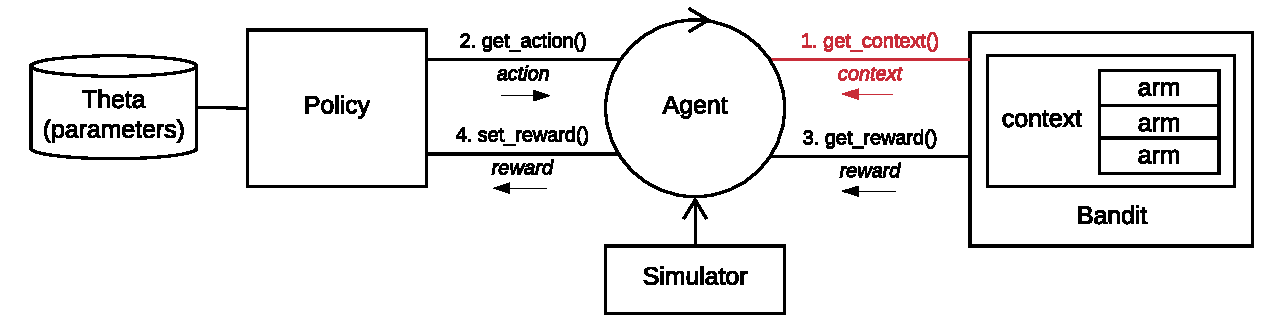
\includegraphics[width=.99\textwidth]{fig/cmab_chart}
    \label{fig:cmab_chart}
      \caption{Diagram of \pkg{contextual}'s basic structure. The context feature vector returned by get\_context() (colored red in the figure) is only taken into account by cMAB policies, and is ignored by MAB policies.}
\end{figure}

On running the \code{Simulator} it starts several (by default, the number of CPU cores minus one) worker processes, splitting simulations as efficiently as possible over each parallell worker. For each simulation, for every time step \code{t}, an \code{agent} clone then loops through each of the four function calls that constitute its main interior loop. Though we will delve deeper into the setup of each of \pkg{contextual}'s main classes in section 3, the current overview enables us to demonstrate how these four function calls relate to the four steps we defined in our cMAB formalization in section 2.1:

\begin{enumerate}
         \item[1)] \code{agent} calls \code{bandit$get_context(t)}, which returns named list \code{list(k = n_arms, d = n_features, X = context)} containing the current \code{d} dimensional \code{context} feature vector \code{X} together with the number of arms \code{k}.
         \item[2)] \code{agent} calls \code{policy$get_action(t, X)}, whereupon \code{policy} relays which arm to play based on the current \code{context} vector \code{X} (in MAB policies, X is ignored) and \code{theta} (the named list holding the parameters summarizing past \code{context}s, \code{action}s and \code{reward}s). \code{policy} then returns a named list \code{list(choice = arm_chosen_by_policy)} that holds the index of the arm to play.
         \item[3)] \code{agent} calls \code{bandit$get_reward(t, context, action)}, which returns a named list \code{list(reward = reward_for_choice_made, optimal_reward_value = optimal_reward_value)} that contains the \code{reward} for the \code{action} returned by \code{policy} in [2] and, optionally, the \code{optimal} reward at the current time \code{t} --- if and when known.
         \item[4)] \code{agent} calls \code{policy$set_reward(t, context, action, reward)} and uses the \code{action} taken, the \code{reward} received, and the current \code{context} to update the set of parameter values in \code{theta}
\end{enumerate}

On completion of all of its simulation runs, \code{Simulator} returns an \code{history} object that contains a complete log of all interactions, which can, among others, be printed, plotted, or summarized:

\begin{knitrout}\small
\definecolor{shadecolor}{rgb}{0.969, 0.969, 0.969}\color{fgcolor}\begin{kframe}
\begin{alltt}
\hlkwd{summary}(history)

\hlcom{## Cumulative Regret}

        agent   cum  cum_var   cum_sd   cum_ci   t
EpsilonGreedy   9.9 116.9596 10.81479 2.119659 100

\hlcom{## Cumulative Reward}

        agent   cum  cum_var   cum_sd   cum_ci   t
EpsilonGreedy 79.44 124.7741 11.17023 2.189326 100
\end{alltt}
\end{kframe}
\end{knitrout}

\section{R6 class structure}

Since it is the \pkg{contextual}'s explicit goal to offer researchers and developers an easily extensible framework to develop, test and compare their own \code{Policy} and \code{Bandit} implementations, the current section offers additional background information on \pkg{contextual}' class structure---both on the R6 class system and on each of the six previously introduced core \pkg{contextual} classes.

\subsection{R and the R6 Class System}

Statistical computational methods, in R or otherwise, are regularly made available through single-use scripts or basic, isolated code packages. Usually, such code examples are meant to give a basic idea of a statistical method, technique or algorithm in the context of a scientific paper.  Such code examples offer their scientific audience a rough inroad towards the comparison and further implementation of their underlying methods. However, when a set of well-researched interrelated algorithms, such as MAB and cMAB policies, find growing academic, practical and commercial adoption, it becomes crucial to offer a more standardized and more accessible way to compare such methods and algorithms.

It is against this background that we decided to develop the \pkg{contextual} R package---a package that would offer an easily extendible and open bandit framework together with extensible bandit and policy libraries. To us, it made the most sense to create such a package in R, as R is currently the de facto language for the dissemination of new statistical methods, techniques, and algorithms---while it is at the same time finding ever-growing adoption in industry. The resulting lively exchange of R related code, data, and knowledge between scientists and practitioners offers precisely the kind of cross-pollination that \pkg{contextual} hopes to facilitate.

Though widely used as a procedural language, R offers several Object Oriented (OO) systems, which can significantly help in structuring the development of more complex packages. Out of the OO systems available (S3, S4, R5 and R6), we settled on R6, as it offered several advantages compared to the other options. Firstly, it implements a mature object-oriented design when compared to S3. Secondly, its classes can be accessed and modified by reference---which offers the added advantage that R6 classes are instantly recognizable for developers with a background in \proglang{Java} or \proglang{C++}. Finally, when compared to the older R5 reference class system, R6 classes are lighter-weight and (as they do not make use of S4 classes) do not require the methods package---which makes \pkg{contextual} substantially less resource-hungry than it would otherwise have been.

\subsection{Main classes}

In this section, we go over each of \pkg{contextual}'s six main classes in some more detail---with an emphasis on the Bandit and Policy classes. To clarify \pkg{contextual}'s class structure, we also include two UML diagrams (UML or "Unified Modeling Language" is a modeling language that presents a standard way to visualize the overall class structure and general design of a software application or framework). The UML class diagram shown in Figure \ref{fig:contextual_class} on page \pageref{fig:contextual_class} visualizes \pkg{contextual}'s static object model, showing how its classes inherit from, and interface with, each other. The UML sequence diagram in figure Figure \ref{fig:contextual_sequence} on page \pageref{fig:contextual_sequence}, on the other hand, illustrates how \pkg{contextual}'s classes interact dynamically over time.

\subsubsection{Bandit}

In \pkg{contextual}, any bandit implementation is expected to subclass and extend the Bandit superclass. It is then up to these subclasses themselves to provide an implementation for each of its abstract methods.\code{Bandit} subclasses are furthermore expected to set instance variable \code{self\$k} to the number of arms, and \code{self\$d} to the number of context features. On meeting this requirement, a \code{Bandit} is then required to implement \code{get_context()} and \code{do_action()}:

\begin{knitrout}\small
\definecolor{shadecolor}{rgb}{0.969, 0.969, 0.969}\color{fgcolor}\begin{kframe}
\begin{alltt}
Bandit <- R6::\hlkwd{R6Class}(
  public = \hlkwd{list}(
    k             = NULL,  \hlcom{# number of \hlkwd{arms} (integer)}
    d             = NULL,  \hlcom{# dimension of context \hlkwd{feature} (integer)}
    precaching    = FALSE, \hlcom{# pregenerate context & reward matrices? (boolean)}

    get_context = \hlkwd{function}(t) \{
      \hlkwd{stop}(\hlstr{"Bandit subclass needs to implement bandit$\hlkwd{get_context}()"})
\hlcom{      # return a list with self$k, self$d and, where applicable, context matrix X.}
      \hlkwd{list}(k = n_arms, d = n_features, X = context)
    \},
    get_reward = \hlkwd{function}(t, context, action) \{
      \hlkwd{stop}(\hlstr{"Bandit subclass needs to implement bandit$\hlkwd{do_action}()"})
\hlcom{      # return a list with the reward and, if known, the reward of the best arm.}
      \hlkwd{list}(reward = reward_for_choice_made, optimal = optimal_reward)
    \},
    generate_bandit_data = \hlkwd{function}(n) \{
\hlcom{      # called when precaching is TRUE. Pregenerates contexts and rewards.}
      \hlkwd{stop}("Bandit subclass needs to implement bandit$\hlkwd{generate_cache}()
           when bandit$precaching is TRUE.",
    \}
  )
)
\end{alltt}
\end{kframe}
\end{knitrout}


Bandit's functions can be described as follows:

\begin{itemize}
  \item{\code{new()}}{ Generates and initializes a new \code{Bandit} object. }
  \item{\code{pre_calculate()}}{
     Called right after \code{Simulator} sets its seed,
     but before it starts iterating over all time steps \code{t} in T. If you need to initialize random values in a \code{Policy},
     this is the place to do so.
  }
  \item{\code{get_context(t)}}{
     Returns a named list \code{list(k = n_arms, d = n_features, X = context)}
     with the current \code{d} dimensional \code{context} feature vector \code{X} together with the number of arms \code{k}.
 }
  \item{\code{get_reward(t, context, action)}}{
     Returns the named list \code{list(reward = reward_for_choice_made,
     optimal = optimal_reward_value)} containing the \code{reward}
     for the \code{action} previously returned by \code{policy} and,
     optionally, the \code{optimal} reward
     at the current time \code{t}.
 }
  \item{\code{generate_bandit_data()}}{
     A helper function that is called before \code{Simulator} starts iterating over all time steps \code{t} in T.
     This function is called when \code{bandit$precaching} has been set to \code{TRUE}.
     Pregenerate \code{contexts} and \code{rewards} here.
  }
\end{itemize}

Where possible, it is advisable to pregenerate or precache \code{Bandit} contexts and rewards, as this is (as is generally the case in R) computationally much more efficient than the repeated generation of reward vectors and context matrices. This pregeneration can be implemented in \code{generate_bandit_data()}. It is called during a \code{Bandit}'s initialization---if and when the \code{Bandit}'s \code{self$precaching} variable is \code{TRUE}.

We also made several \code{Bandit} subclasses available. For each Bandit, there is at least one example script, to be found in the package’s demo directory:

\begin{itemize}
         \item \code{BasicBandit}: this basic (non-contextual) k-armed bandit synthetically generates rewards based on a weight vector. It returns a unit vector for context matrix X.
                  \item \code{SyntheticBandit}: an example of a more complex and versatile synthetic bandit. It pregenerates both a randomized context matrix and reward vectors
         \item \code{ContextualBandit}: a contextual bandit that synthetically generates contextual rewards based on randomly set weights. It can simulate mixed user (cross-arm) and article (arm) feature vectors, generated from parameters k, d and num\_users.
         \item \code{ContinuumBandit}: a basic example of a continuum bandit.
         \item \code{LiBandit}: a basic example of a bandit that makes use of offline data - here, an implementation of Li's [reference].
\end{itemize}

Each of these bandits can be used to run policies without further ado. They can, however, also be used as superclasses for custom \code{Bandit} subclas implementations. Or as templates for \code{Bandit} implementation(s) that directly subclass \pkg{contextual}'s \code{Bandit} superclass.

\subsubsection{Policy}

\code{Policy} is another central and often subclassed contexual superclass. Just like \code{Bandit}, this abstract class declares methods without itself offering an implementation. Any \code{Policy} subclass is therefore expected to implement \code{get_action()} and \code{set_reward()}. Also, any parameters that keep track or summarize \code{context}, \code{action} and \code{reward} values are required to be saved to \code{Policy}'s public named list \code{theta}.

\begin{knitrout}\small
\definecolor{shadecolor}{rgb}{0.969, 0.969, 0.969}\color{fgcolor}\begin{kframe}
\begin{alltt}
\hlstd{Policy} \hlkwb{<-} \hlstd{R6}\hlopt{::}\hlkwd{R6Class}\hlstd{(}
  \hlkwc{public} \hlstd{=} \hlkwd{list}\hlstd{(}
    \hlkwc{name}          \hlstd{=} \hlstr{""}\hlstd{,}
    \hlkwc{action}        \hlstd{=} \hlkwa{NULL}\hlstd{,}    \hlcom{# action list}
    \hlkwc{theta}         \hlstd{=} \hlkwa{NULL}\hlstd{,}    \hlcom{# list of all parameters theta}
    \hlkwc{theta_to_arms} \hlstd{=} \hlkwa{NULL}\hlstd{,}    \hlcom{# theta to arms list}
    \hlkwc{initialize} \hlstd{=} \hlkwa{function}\hlstd{(}\hlkwc{name} \hlstd{=} \hlstr{"Not implemented"}\hlstd{) \{}
      \hlstd{self}\hlopt{$}\hlstd{name}   \hlkwb{<-} \hlstd{name}    \hlcom{# each policy has a name}
      \hlstd{self}\hlopt{$}\hlstd{theta}  \hlkwb{<-} \hlkwd{list}\hlstd{()}  \hlcom{# list that keeps track of all parameter values}
      \hlstd{self}\hlopt{$}\hlstd{action} \hlkwb{<-} \hlkwd{list}\hlstd{()}  \hlcom{# initiatlisation of action list for internal use}
    \hlstd{\},}
    \hlkwc{get_action} \hlstd{=} \hlkwa{function}\hlstd{(}\hlkwc{t}\hlstd{,} \hlkwc{context}\hlstd{) \{}
      \hlcom{# chooses arm based on theta and context, returns its index in action$choice}
      \hlkwd{stop}\hlstd{(}\hlstr{"Policy$get_action() has not been implemented."}\hlstd{,} \hlkwc{call.} \hlstd{=} \hlnum{FALSE}\hlstd{)}
    \hlstd{\},}
    \hlkwc{set_reward} \hlstd{=} \hlkwa{function}\hlstd{(}\hlkwc{t}\hlstd{,} \hlkwc{context}\hlstd{,} \hlkwc{action}\hlstd{,} \hlkwc{reward}\hlstd{) \{}
      \hlcom{# updates parameters in theta based on reward awarded by bandit to chosen arm}
      \hlkwd{stop}\hlstd{(}\hlstr{"Policy$set_reward() has not been implemented."}\hlstd{,} \hlkwc{call.} \hlstd{=} \hlnum{FALSE}\hlstd{)}
    \hlstd{\},}
    \hlkwc{set_parameters} \hlstd{=} \hlkwa{function}\hlstd{() \{}
      \hlcom{# policy parameters (not theta!) initialization happens here}
      \hlkwd{stop}\hlstd{(}\hlstr{"Policy$set_parameters() has not been implemented."}\hlstd{,} \hlkwc{call.} \hlstd{=} \hlnum{FALSE}\hlstd{)}
    \hlstd{\},}
    \hlkwc{initialize_theta} \hlstd{=} \hlkwa{function}\hlstd{() \{}
      \hlcom{# implementation not shown - called during contextual's initialisation}
      \hlcom{# copies theta_to_arms k times, makes the copies available through theta}
    \hlstd{\}}
  \hlstd{)}
\hlstd{)}
\end{alltt}
\end{kframe}
\end{knitrout}

Bandit's functions can be described as following:

\begin{itemize}

\item{\code{set_parameters()}}{
 This helper function, called during a Policy's initialisation, assigns the values
 it finds in list \code{self$theta_to_arms} to each of the Policy's k arms.
 The parameters defined here can then be accessed by arm index in the following way:
 \code{theta[[index_of_arm]]$parameter_name}.
}

\item{\code{get_action(t, context)}}{
 Calculates which arm to play based on the current values in named list \code{theta}
 and the current \code{context}. Returns a named list
 \code{list(choice = arm_chosen_by_policy)} that holds the index of the arm
 to play.
}

\item{\code{set_reward(t, context, action, reward)}}{
 Returns the named list
 \code{list(reward = reward_for_choice_made, optimal = optimal_reward_value)} containing the \code{reward}
 for the \code{action} previously returned by \code{policy} and, optionally, the \code{optimal} reward
 at the current time \code{t}.
 }
\end{itemize}

\subsubsection{Agent}

To ease the encapsulation of parallel \code{Bandit} and \code{Policy} simulations, \code{Agent} is responsibe for the flow of information between and the running of one \code{Bandit} and \code{Policy} pair, for example:

\begin{knitrout}\small
\definecolor{shadecolor}{rgb}{0.969, 0.969, 0.969}\color{fgcolor}\begin{kframe}
\begin{alltt}
\hlstd{policy}             \hlkwb{<-} \hlstd{EpsilonGreedyPolicy}\hlopt{$}\hlkwd{new}\hlstd{(}\hlkwc{epsilon} \hlstd{=} \hlnum{0.1}\hlstd{,} \hlkwc{name} \hlstd{=} \hlstr{"EG"}\hlstd{)}
\hlstd{bandit}             \hlkwb{<-} \hlstd{SyntheticBandit}\hlopt{$}\hlkwd{new}\hlstd{(}\hlkwc{weights} \hlstd{=} \hlkwd{c}\hlstd{(}\hlnum{0.9}\hlstd{,} \hlnum{0.1}\hlstd{,} \hlnum{0.1}\hlstd{))}
\hlstd{agent}              \hlkwb{<-} \hlstd{Agent}\hlopt{$}\hlkwd{new}\hlstd{(policy,bandit)}
\end{alltt}
\end{kframe}
\end{knitrout}

It does this by keeping track of \code{t}  through its private named list variable \code{state} and by making sure that, at each time step \code{t}, all four main \code{Bandit} and \code{Policy} cMAB methods are called in correct order:

\begin{knitrout}\small
\definecolor{shadecolor}{rgb}{0.969, 0.969, 0.969}\color{fgcolor}\begin{kframe}
\begin{alltt}
\hlstd{Agent} \hlkwb{<-} \hlstd{R6}\hlopt{::}\hlkwd{R6Class}\hlstd{(}
  \hlkwc{public} \hlstd{=} \hlkwd{list}\hlstd{(}
    \hlcom{#...}
    \hlkwc{do_step} \hlstd{=} \hlkwa{function}\hlstd{() \{}
      \hlstd{private}\hlopt{$}\hlstd{t} \hlkwb{<-} \hlstd{private}\hlopt{$}\hlstd{t} \hlopt{+} \hlnum{1}
      \hlstd{context} \hlkwb{=} \hlstd{bandit}\hlopt{$}\hlkwd{get_context}\hlstd{(private}\hlopt{$}\hlstd{t)}
      \hlstd{action}  \hlkwb{=} \hlstd{policy}\hlopt{$}\hlkwd{get_action} \hlstd{(private}\hlopt{$}\hlstd{t, context)}
      \hlstd{reward}  \hlkwb{=} \hlstd{bandit}\hlopt{$}\hlkwd{get_reward} \hlstd{(private}\hlopt{$}\hlstd{t, context, action)}
      \hlstd{theta}   \hlkwb{=} \hlstd{policy}\hlopt{$}\hlkwd{set_reward} \hlstd{(private}\hlopt{$}\hlstd{t, context, action, reward)}
      \hlkwd{list}\hlstd{(}\hlkwc{context} \hlstd{= context,} \hlkwc{action} \hlstd{= action,} \hlkwc{reward} \hlstd{= reward,}\hlkwc{theta} \hlstd{= theta)}
    \hlstd{\}}
    \hlcom{#...}
  \hlstd{)}
\hlstd{)}
\end{alltt}
\end{kframe}
\end{knitrout}

Its main function is \code{do_step()}, generally called by the worker of a \code{Simulator} object that takes care of the running of a particular \code{agent} instance:

\begin{itemize}
   \item{\code{do_step()}}{
      Completes one time step \code{t} by consecutively calling
      \code{bandit$get_context()}, \code{policy$get_action()}, \code{bandit$get_reward()} and \code{policy$set_reward()}.
    }
\end{itemize}

\subsubsection{Simulator}

A Simulator instance is the entry point of any \pkg{contextual} simulation. It encapsulates one or more \code{Agents}, clones them if necessary, runs the \code{Agents} (in parallel, by default), and saves the log of all of the \code{Agents} interactions to a \code{History} object:

\begin{knitrout}\small
\definecolor{shadecolor}{rgb}{0.969, 0.969, 0.969}\color{fgcolor}\begin{kframe}
\begin{alltt}
\hlstd{history} \hlkwb{<-} \hlstd{Simulator}\hlopt{$}\hlkwd{new}\hlstd{(}\hlkwc{agents} \hlstd{= agent,} \hlkwc{horizon} \hlstd{=} \hlnum{10}\hlstd{,} \hlkwc{simulations} \hlstd{=} \hlnum{10}\hlstd{)}\hlopt{$}\hlkwd{run}\hlstd{()}
\end{alltt}
\end{kframe}
\end{knitrout}

By default, for performance reasons, a \code{Simulator} does not save \code{context} matrices and the (potentially deeply nested) \code{theta} list to its \code{History log}. But with its \code{save_context} and \code{save_theta} arguments set to \code{TRUE}, a the above history data.table object would be structured as follows:

\begin{knitrout}\small
\definecolor{shadecolor}{rgb}{0.969, 0.969, 0.969}\color{fgcolor}\begin{kframe}
\begin{alltt}
\hlkwd{print}(history)

 $ t                   : int  1 2 3 4 5 6 7 8 9 10 ...  \hlcom{# time step}
 $ sim                 : int  1 1 1 1 1 1 1 1 1 1 ...   \hlcom{# simulation index number}
 $ choice              : num  3 1 1 1 1 1 1 1 1 1 ...   \hlcom{# arm chosen by policy}
 $ reward              : num  0 1 0 1 1 1 1 1 1 1 ...   \hlcom{# reward awarded by bandit}
 $ choice_is_optimal   : int  0 1 1 1 1 1 1 1 1 1 ...   \hlcom{# chosen arm optimal one?}
 $ optimal_reward_value: num  1 1 0 1 1 1 1 1 1 1 ...   \hlcom{# best reward at t}
 $ propensity          : num  0.9 0.9 0.033 0.9 0.9 ... \hlcom{# propensity of chosen arm}
 $ agent               : chr  \hlstr{'ThompsonSampling'} ...    i\hlcom{# agent name}
 $ context             : List of 100 matrices           \hlcom{# list of context matrices}
 $ theta               : List of 100 Lists              \hlcom{# list \hlkwd{of} (nested) thetas}
\end{alltt}
\end{kframe}
\end{knitrout}

To specify how to run a simulation and which data is to be saved to a \code{Simulator} instance's \code{History} log, a Simulator object can be configured through the following parameters:

\begin{itemize}
   \item{\code{agents}}{
     An \code{Agent} instance, or a \code{list} of \code{Agent} instances to be run by the instantiated \code{Simulator}.
   }
   \item{\code{horizon}}{
     The T time steps to run the instantiated \code{Simulator}.
   }
   \item{\code{simulations}}{
     How many times to repeat each agent's simulation with a new seed on each repeat (itself deterministically derived from set\_seed).
   }
   \item{\code{save_context}}{
     Save context matrices \code{X} to the History log during a simulation?
   }
   \item{\code{save_theta}}{
     Save the parameter list \code{theta} to the History log during a simulation?
   }
   \item{\code{do_parallel}}{
      Run \code{Simulator} processes in parallel?
   }
   \item{\code{worker_max}}{
      Specifies how many parallel workers are to be used, when \code{do_parallel} is \code{TRUE}. If unspecified, the amount of workers defaults to \code{max(workers_available)-1}.
   }
   \item{\code{continuous_counter}}{
      Of use to, among others, offline Bandits.
      If \code{continuous_counter} is set to \code{TRUE}, the current \code{Simulator}
      iterates over all rows in a data set for each repeated simulation.
      If \code{FALSE}, it splits the data into \code{simulations} parts,
      and a different subset of the data for each repeat of an agent's simulation.
   }
   \item{\code{set_seed}}{
      Sets the seed of R's random number generator for the current \code{Simulator}.
   }
   \item{\code{write_progress_file}}{
       If \code{TRUE}, \code{Simulator} writes \code{progress.log} and \code{doparallel.log}
       files to the current working directory, allowing you to keep track of \code{workers}, iterations,
       and potential errors when running a \code{Simulator} in parallel.
   }
   \item{\code{include_packages}}{
       List of packages that (one of) the policies depend on. If a \code{Policy} requires an
       R package to be loaded, this option can be used to load that package on each of the workers.
       Ignored if \code{do_parallel} is \code{FALSE}.
   }
   \item{\code{reindex_t}}{
      If \code{TRUE}, removes empty rows from the \code{History} log,
      re-indexes the \code{t} column, and truncates the resulting data to the shortest simulation
      grouped by agent and simulation.
   }
\end{itemize}

\subsubsection{History}

A \code{Simulator} aggregates the data acquired during a simulation in a \code{History} object's private \code{data.table} log. It also calculates per agent average cumulative reward, and, when the optimal outcome per \code{t} is known, per agent average cumulative regret. It is furthermore possible to \code{plot()} a \code{History object}, \code{summarize()} it, and, among others, obtain either a \code{data.frame()} or a \code{data.table()} from any \code{History} instance:

\begin{knitrout}\small
\definecolor{shadecolor}{rgb}{0.969, 0.969, 0.969}\color{fgcolor}\begin{kframe}
\begin{alltt}
\hlstd{history}             \hlkwb{<-} \hlstd{Simulator}\hlopt{$}\hlkwd{new}\hlstd{(agent)}\hlopt{$}\hlkwd{run}\hlstd{()}
\hlstd{dt}                  \hlkwb{<-} \hlstd{history}\hlopt{$}\hlkwd{get_data_table}\hlstd{()}
\hlstd{df}                  \hlkwb{<-} \hlstd{history}\hlopt{$}\hlkwd{get_data_frame}\hlstd{()}
\hlstd{cumulative_regret}   \hlkwb{<-} \hlstd{history}\hlopt{$}\hlkwd{cumulative}\hlstd{(}\hlkwc{regret} \hlstd{=} \hlnum{TRUE}\hlstd{)}
\end{alltt}
\end{kframe}
\end{knitrout}

Some other History functions:

\begin{itemize}
 \item{\code{save(index,
                  t,
                  action,
                  reward,
                  policy_name,
                  simulation_index,
                  context_value = NA,
                  theta_value = NA)}}{
    Saves one row of simulation data. \code{save()} is generally not called directly, but trough a \code{Simulator} instance.
 }
 \item{\code{save_data(filename = NA)}}{
    Writes the \code{History} log file in its default data.table format,
    with \code{filename} as the name of the file which the data is to be written to.
 }
 \item{\code{load_data = function(filename, nth_rows = 0)}}{
    Reads a \code{History} log file in its default \code{data.table} format,
    with \code{filename} as the name of the file which the data are to be read from.
    If \code{nth_rows} is larger than 0, every \code{nth_rows} of data is read instead of the
    full data file. This can be of use with (a first) analysis of very large data files.
 }
 \item{\code{reindex_t(truncate = TRUE)}}{
    Removes empty rows from the \code{History} log, reindexes the \code{t} column, and,
    if \code{truncate} is \code{TRUE}, truncates the resulting data to the shortest simulation
    grouped by agent and simulation.
 }
 \item{\code{print_data()}}{
    Prints a summary of the \code{History} log.
 }
 \item{\code{cumulative(final = TRUE, regret = TRUE, rate = FALSE)}}{
    Returns cumulative reward (when \code{regret} is \code{FALSE}) or regret. When \code{final} is \code{TRUE},
    it only returns the final value. When \code{final} is FALSE, it returns a \code{data.table} containing all
    cumulative reward or regret values from 1 to T.
    When \code{rate} is \code{TRUE}, cumulative reward or regret are divided by column \code{t} before any values
    are returned.
 }
\end{itemize}

\subsubsection{Plot}

The \code{Plot} class takes an \code{History} object, and offers several default types of plot:

\begin{itemize}
         \item \code{average}: plots the average reward or regret over all simulations per Agent (that is, each Bandit and Policy combo) over time.
         \item \code{cumulative}: plots the average reward or regret over all simulations per Agent over time.
         \item \code{optimal}: if data on optimal choice is available, "optimal" plots how often the best or optimal arm was chosen on average at each timestep, in percentages, over all simulations per Agent.
         \item \code{arms}: plots ratio of arms chosen on average at each time step, in percentages, totaling 100%.

\end{itemize}

\code{Plot} objects can be instantiated directly, or, more commonly, by calling the \code{plot()} function. In either case, make sure to specify a \code{History} instance and one of the plot types specified above:

\begin{knitrout}\small
\definecolor{shadecolor}{rgb}{0.969, 0.969, 0.969}\color{fgcolor}\begin{kframe}
\begin{alltt}
\hlcom{# plot a history object through default generic plot() function}
\hlkwd{plot}\hlstd{(history,} \hlkwc{type} \hlstd{=} \hlstr{"arms"}\hlstd{)}

\hlcom{# or use the Plot class directly}
\hlstd{p1} \hlkwb{<-} \hlstd{Plot}\hlopt{$}\hlkwd{new}\hlstd{()}\hlopt{$}\hlkwd{cumulative}\hlstd{(history)}
\hlstd{p2} \hlkwb{<-} \hlstd{Plot}\hlopt{$}\hlkwd{new}\hlstd{()}\hlopt{$}\hlkwd{average}\hlstd{(history)}
\end{alltt}
\end{kframe}
\end{knitrout}

It is also possible to retrieve a \code{data.frame} object from an \code{History} object, and plot the data in any other way, for instance through ggplot2 (with 95\% confidence interval):

\begin{knitrout}\small
\definecolor{shadecolor}{rgb}{0.969, 0.969, 0.969}\color{fgcolor}\begin{kframe}
\begin{alltt}
\hlstd{bandit}  \hlkwb{<-} \hlstd{ContextualBandit}\hlopt{$}\hlkwd{new}\hlstd{(}\hlkwc{k} \hlstd{=} \hlnum{5}\hlstd{,} \hlkwc{d} \hlstd{=} \hlnum{6}\hlstd{,} \hlkwc{num_users} \hlstd{=} \hlnum{7}\hlstd{)}
\hlstd{agents}  \hlkwb{<-} \hlkwd{list}\hlstd{(}
  \hlstd{Agent}\hlopt{$}\hlkwd{new}\hlstd{(EpsilonGreedyPolicy}\hlopt{$}\hlkwd{new}\hlstd{(}\hlnum{0.1}\hlstd{,} \hlstr{"\textbackslash{}U190-greedy"}\hlstd{), bandit),}
  \hlstd{Agent}\hlopt{$}\hlkwd{new}\hlstd{(ContextualThompsonSamplingPolicy}\hlopt{$}\hlkwd{new}\hlstd{(}\hlkwc{name} \hlstd{=} \hlstr{"ContextualTS"}\hlstd{), bandit),}
  \hlstd{Agent}\hlopt{$}\hlkwd{new}\hlstd{(LinUCBDisjointPolicy}\hlopt{$}\hlkwd{new}\hlstd{(}\hlnum{0.7}\hlstd{,} \hlstr{"LinUCBDisjoint"}\hlstd{), bandit),}
  \hlstd{Agent}\hlopt{$}\hlkwd{new}\hlstd{(LinUCBHybridPolicy}\hlopt{$}\hlkwd{new}\hlstd{(}\hlnum{0.7}\hlstd{,} \hlnum{6}\hlstd{,} \hlstr{"LinUCBHybrid"}\hlstd{), bandit)}
\hlstd{)}
\hlstd{history} \hlkwb{<-} \hlstd{Simulator}\hlopt{$}\hlkwd{new}\hlstd{(agents,} \hlnum{300}\hlstd{,} \hlnum{100}\hlstd{)}\hlopt{$}\hlkwd{run}\hlstd{()}

\hlcom{# plot using contextual - faster, less code and configuration}
\hlkwd{plot}\hlstd{(history,} \hlkwc{type} \hlstd{=} \hlstr{"cumulative"}\hlstd{,} \hlkwc{ci} \hlstd{=} \hlnum{TRUE}\hlstd{,} \hlkwc{rate} \hlstd{=} \hlnum{TRUE}\hlstd{)}
\end{alltt}
\end{kframe}
\end{knitrout}
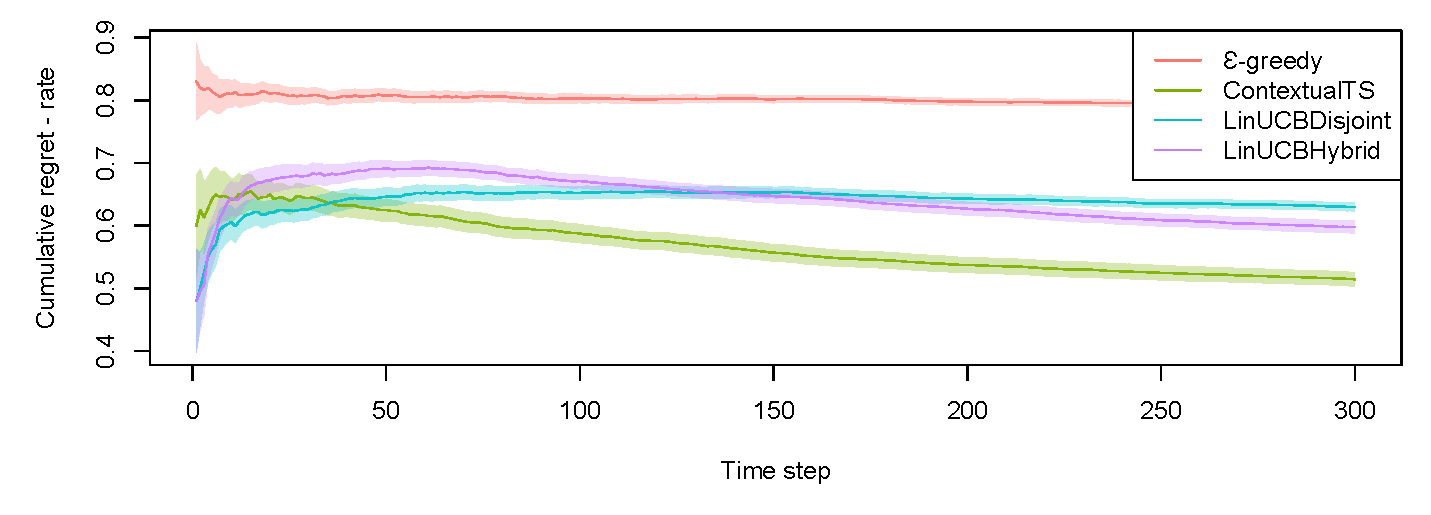
\includegraphics[width=\textwidth]{fig/contextual_plotclass}
\begin{knitrout}\small
\definecolor{shadecolor}{rgb}{0.969, 0.969, 0.969}\color{fgcolor}\begin{kframe}
\begin{alltt}
\hlcom{# plot using library(ggplot2) - more code and configuration, also more flexible}

\hlstd{dt}        \hlkwb{<-} \hlstd{history}\hlopt{$}\hlkwd{get_data_table}\hlstd{()}
\hlstd{max_sim}   \hlkwb{<-} \hlstd{dt[,}\hlkwd{max}\hlstd{(sim)]}
\hlstd{dt}\hlopt{$}\hlstd{cumsum} \hlkwb{<-} \hlstd{dt[,}\hlkwd{cumsum}\hlstd{(optimal_reward_value} \hlopt{-} \hlstd{reward)}\hlopt{/}\hlstd{t,} \hlkwc{by} \hlstd{=} \hlkwd{list}\hlstd{(agent, sim)]}\hlopt{$}\hlstd{V1}
\hlstd{cs}        \hlkwb{<-} \hlstd{dt[,}\hlkwd{list}\hlstd{(}\hlkwc{sd} \hlstd{=} \hlkwd{sd}\hlstd{(cumsum),} \hlkwc{mean} \hlstd{=} \hlkwd{mean}\hlstd{(cumsum)),} \hlkwc{by} \hlstd{=} \hlkwd{list}\hlstd{(t, agent)]}
\hlstd{ci_range}  \hlkwb{<-} \hlstd{cs}\hlopt{$}\hlstd{mean} \hlopt{+} \hlkwd{outer}\hlstd{(cs}\hlopt{$}\hlstd{sd}\hlopt{/}\hlkwd{sqrt}\hlstd{(max_sim),} \hlkwd{c}\hlstd{(}\hlnum{1.96}\hlstd{,} \hlopt{-}\hlnum{1.96}\hlstd{))}
\hlstd{cs}        \hlkwb{<-} \hlkwd{cbind}\hlstd{(cs, ci_range)}
\hlstd{p}         \hlkwb{<-} \hlkwd{ggplot}\hlstd{(}\hlkwc{data} \hlstd{= cs,} \hlkwd{aes}\hlstd{(}\hlkwc{x} \hlstd{= t,} \hlkwc{y} \hlstd{= mean,} \hlkwc{ymin} \hlstd{= V1,} \hlkwc{ymax} \hlstd{= V2))} \hlopt{+}
             \hlkwd{geom_line}\hlstd{(}\hlkwd{aes}\hlstd{(}\hlkwc{color} \hlstd{= agent))} \hlopt{+}
             \hlkwd{geom_ribbon}\hlstd{(}\hlkwd{aes}\hlstd{(}\hlkwc{fill} \hlstd{= agent),} \hlkwc{alpha} \hlstd{=} \hlnum{0.3}\hlstd{)} \hlopt{+}
             \hlkwd{theme}\hlstd{(}\hlkwc{legend.justification} \hlstd{=} \hlkwd{c}\hlstd{(}\hlnum{0}\hlstd{,}\hlnum{0}\hlstd{),} \hlkwc{legend.position} \hlstd{=} \hlkwd{c}\hlstd{(}\hlnum{0.8}\hlstd{,}\hlnum{0.6}\hlstd{),}
                   \hlkwc{legend.title} \hlstd{=} \hlkwd{element_blank}\hlstd{())} \hlopt{+}
             \hlkwd{labs}\hlstd{(}\hlkwc{x} \hlstd{=} \hlstr{"Time step"}\hlstd{,} \hlkwc{y} \hlstd{=} \hlstr{"Cumulative regret - rate"}\hlstd{)}
\hlkwd{print}\hlstd{(p)}
\end{alltt}
\end{kframe}
\end{knitrout}
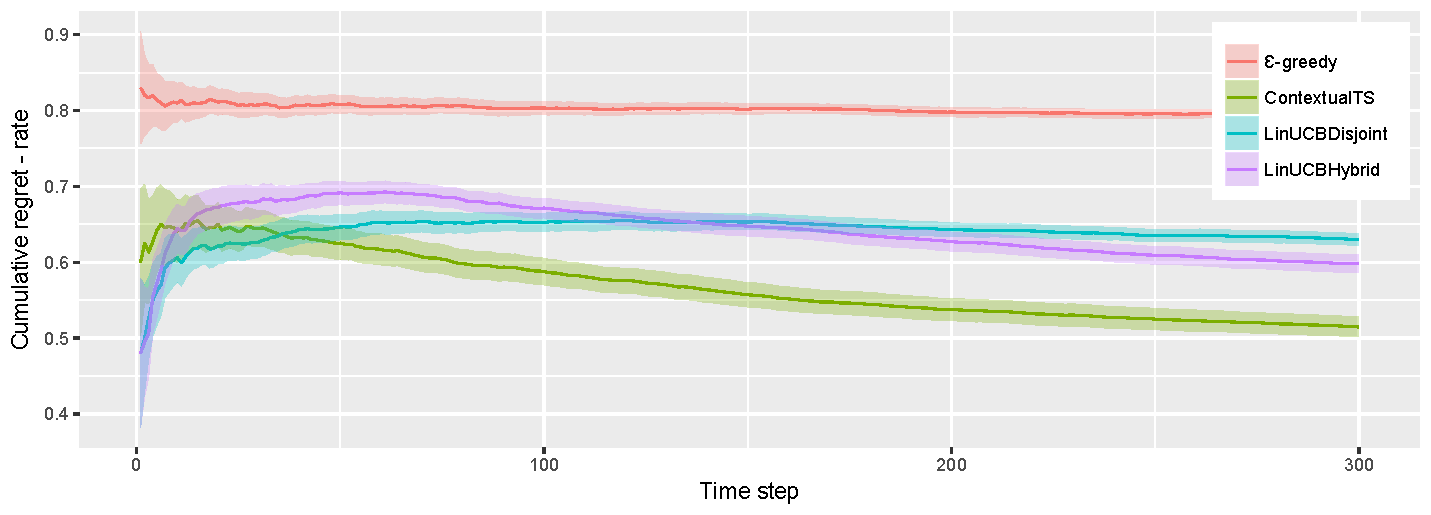
\includegraphics[width=\textwidth]{fig/contextual_ggplot}

\section{Implementing and extending Policy and Bandit subclasses}

Though section 3 provides an introduction to all of \pkg{contextual}'s main classes, in practice, researchers will mostly focus on subclassing \code{Policies} and \code{Bandits}. The current section therefore first demonstrates how to implement some well-known bandit algorithms, and, secondly, how to create \code{Policy} and \code{Bandit} sub-subclasses.

\subsection{BasicBandit: a Minimal Bernoulli Bandit}

Where not otherwise noted, all \code{Bandit} implementations in the current paper refer to (or will be configured as) multi-armed \code{Bandits} with Bernoulli rewards. For Bernoulli \code{Bandits}, the reward received is either a zero or a one: on each $t$ they offer either a reward of $1$ with probability $p$ or a reward of $0$ with probability $p - 1$. In other words, a Bernoulli Bandit has a finite set of arms a \(  \in \left\{ 1, \dots, k \right\} \) where the rewards for each arm $a$ is distributed Bernoulli with parameter ${\mu}a$, the expected reward of the arm.

One example of a very simple non-contextual Bernoulli bandit is \pkg{contextual}'s minimal \code{Bandit} implementation, \code{BasicBandit}:

\begin{knitrout}\small
\definecolor{shadecolor}{rgb}{0.969, 0.969, 0.969}\color{fgcolor}\begin{kframe}
\begin{alltt}
\hlstd{BasicBandit} \hlkwb{<-} \hlstd{R6}\hlopt{::}\hlkwd{R6Class}\hlstd{(}
  \hlkwc{inherit} \hlstd{= Bandit,}
  \hlkwc{public} \hlstd{=} \hlkwd{list}\hlstd{(}
    \hlkwc{initialize}   \hlstd{=} \hlkwa{function}\hlstd{(}\hlkwc{weights} \hlstd{=} \hlkwa{NULL}\hlstd{) \{}
      \hlstd{self}\hlopt{$}\hlkwd{set_weights}\hlstd{(weights)}                         \hlcom{# arm weight vector}
      \hlstd{private}\hlopt{$}\hlstd{X} \hlkwb{<-} \hlkwd{array}\hlstd{(}\hlnum{1}\hlstd{,} \hlkwc{dim} \hlstd{=} \hlkwd{c}\hlstd{(self}\hlopt{$}\hlstd{d, self}\hlopt{$}\hlstd{k,} \hlnum{1}\hlstd{))} \hlcom{# context matrix of ones}
    \hlstd{\},}
    \hlcom{# ...}
    \hlkwc{get_weights} \hlstd{=} \hlkwa{function}\hlstd{() \{}
      \hlstd{private}\hlopt{$}\hlstd{W}
    \hlstd{\},}
    \hlkwc{set_weights} \hlstd{=} \hlkwa{function}\hlstd{(}\hlkwc{local_W}\hlstd{) \{}
      \hlstd{private}\hlopt{$}\hlstd{W} \hlkwb{<-} \hlkwd{matrix}\hlstd{(local_W,} \hlkwc{nrow} \hlstd{=} \hlnum{1L}\hlstd{)}           \hlcom{# arm weight vector}
      \hlstd{self}\hlopt{$}\hlstd{d}    \hlkwb{<-} \hlkwd{as.integer}\hlstd{(}\hlkwd{dim}\hlstd{(private}\hlopt{$}\hlstd{W)[}\hlnum{1}\hlstd{])}        \hlcom{# context dimensions}
      \hlstd{self}\hlopt{$}\hlstd{k}    \hlkwb{<-} \hlkwd{as.integer}\hlstd{(}\hlkwd{dim}\hlstd{(private}\hlopt{$}\hlstd{W)[}\hlnum{2}\hlstd{])}        \hlcom{# arms}
      \hlstd{private}\hlopt{$}\hlstd{W}
    \hlstd{\},}
    \hlkwc{get_context} \hlstd{=} \hlkwa{function}\hlstd{(}\hlkwc{t}\hlstd{) \{}
      \hlstd{contextlist} \hlkwb{<-} \hlkwd{list}\hlstd{(}\hlkwc{k} \hlstd{= self}\hlopt{$}\hlstd{k,} \hlkwc{d} \hlstd{= self}\hlopt{$}\hlstd{d,} \hlkwc{X} \hlstd{= private}\hlopt{$}\hlstd{X)}
      \hlstd{contextlist}
    \hlstd{\},}
    \hlkwc{get_reward} \hlstd{=} \hlkwa{function}\hlstd{(}\hlkwc{t}\hlstd{,} \hlkwc{context}\hlstd{,} \hlkwc{action}\hlstd{) \{}
      \hlstd{private}\hlopt{$}\hlstd{R}  \hlkwb{<-} \hlkwd{as.double}\hlstd{(}\hlkwd{matrix}\hlstd{(}\hlkwd{runif}\hlstd{(self}\hlopt{$}\hlstd{k)} \hlopt{<} \hlkwd{get_weights}\hlstd{(), self}\hlopt{$}\hlstd{k, self}\hlopt{$}\hlstd{d))}
      \hlstd{rewardlist} \hlkwb{<-} \hlkwd{list}\hlstd{(}
        \hlkwc{reward}                   \hlstd{= private}\hlopt{$}\hlstd{R[action}\hlopt{$}\hlstd{choice],}
        \hlkwc{optimal_reward_value}     \hlstd{= private}\hlopt{$}\hlstd{R[}\hlkwd{which.max}\hlstd{(private}\hlopt{$}\hlstd{R)]}
      \hlstd{)}
      \hlstd{rewardlist}
    \hlstd{\}}
    \hlcom{# ...}
  \hlstd{)}
\hlstd{)}
\end{alltt}
\end{kframe}
\end{knitrout}

\code{BasicBandit} expects a \code{weight} vector of probabilities, where every element in \code{weight} represents the probability of \code{BasicBandit} returning a reward of $1$ for one of its \code{k} arms. Also, observe that, at every \code{t}, \code{BasicBandit} sets private \code{context} matrix \code{X} to an unchanging, neutral \code{d} features times \code{k} arms unit matrix, which alludes to the fact that \code{BasicBandit} does not generate any covaried contextual cues related to its arms.

\subsection{Epsilon First}

An important feature of \pkg{contextual} is that it eases the conversion from formal and pseudocode policy descriptions to clean R6 classes. We will give several examples of such conversions in the current paper, starting with the implementation of the Epsilon First algorithm. In this non-contextual algorithm, also known as AB(C) testing, a pure exploration phase is followed by a pure exploitation phase.

In that respect, the Epsilon First algorithm is actually equivalent to a randomized controlled trial (RCT). An RCT, generally refered to as the gold standard clinical research paradigm, is a study design where subjects are allocated at random to receive one of several clinical interventions. On completion of an RCT, the most succesful intervention up till that point in time is suggested to be the superior "evidence-based" option from then on.

A more formal pseudocode description of this Epsilon First policy:

\begin{algorithm}[H]
\caption{Epsilon First}
\label{Alg:EpsilonFirst}
\begin{algorithmic}
\REQUIRE \(   \eta \in \mathbb{Z}^{+} \)  , number of time steps $t$ in the exploration phase
\STATE \( n_{a} \leftarrow 0 \) for all arms a \(  \in \left\{ 1, \dots, k \right\} \)  (count how many times an arm has been chosen)
\STATE \( \hat{\mu}_{a} \leftarrow 0 \) for all arms a  \(   \in \left\{ 1, \dots, k \right\} \)  (estimate of expected reward per arm)
% Run through time points:
\FOR{$t=1, \dots, T$}
	% Run through arms. Step 1, select which one to play
	\IF {\(t \leq \eta\)}
	       \STATE play a random arm out of all arms a \(   \in \left\{ 1, \dots, k \right\} \)
	\ELSE
	        \STATE play arm \(a_t = \argmax_a  \hat{\mu}_{t=\eta,a}  \) with ties broken arbitrarily
	\ENDIF
	\STATE observe real-valued payoff $r_t$
	% Update:
	\STATE \( n_{a_{t}} \leftarrow n_{a_{t-1}} + 1  \)
   \STATE \( \hat{\mu}_{t,a_{t}} \leftarrow   \cfrac{r_t - \hat{\mu}_{t-1,a_{t}} }{n_{a_{t}}}   \)
\ENDFOR
\end{algorithmic}
\end{algorithm}

And the above pseudocode converted to an \code{EpsilonFirstPolicy} class:

\begin{knitrout}\small
\definecolor{shadecolor}{rgb}{0.969, 0.969, 0.969}\color{fgcolor}\begin{kframe}
\begin{alltt}
\hlstd{EpsilonFirstPolicy} \hlkwb{<-} \hlstd{R6}\hlopt{::}\hlkwd{R6Class}\hlstd{(}
  \hlkwc{public} \hlstd{=} \hlkwd{list}\hlstd{(}
    \hlkwc{first} \hlstd{=} \hlkwa{NULL}\hlstd{,}
    \hlkwc{initialize} \hlstd{=} \hlkwa{function}\hlstd{(}\hlkwc{first} \hlstd{=} \hlnum{100}\hlstd{,} \hlkwc{name} \hlstd{=} \hlstr{"EpsilonFirst"}\hlstd{) \{}
      \hlstd{super}\hlopt{$}\hlkwd{initialize}\hlstd{(name)}
      \hlstd{self}\hlopt{$}\hlstd{first} \hlkwb{<-} \hlstd{first}
    \hlstd{\},}
    \hlkwc{set_parameters} \hlstd{=} \hlkwa{function}\hlstd{() \{}
      \hlstd{self}\hlopt{$}\hlstd{theta_to_arms} \hlkwb{<-} \hlkwd{list}\hlstd{(}\hlstr{'n'} \hlstd{=} \hlnum{0}\hlstd{,} \hlstr{'mean'} \hlstd{=} \hlnum{0}\hlstd{)}
    \hlstd{\},}
    \hlkwc{get_action} \hlstd{=} \hlkwa{function}\hlstd{(}\hlkwc{context}\hlstd{,} \hlkwc{t}\hlstd{) \{}
      \hlkwa{if} \hlstd{(}\hlkwd{sum_of}\hlstd{(theta}\hlopt{$}\hlstd{n)} \hlopt{<} \hlstd{first) \{}
        \hlstd{action}\hlopt{$}\hlstd{choice}          \hlkwb{<-} \hlkwd{sample.int}\hlstd{(context}\hlopt{$}\hlstd{k,} \hlnum{1}\hlstd{,} \hlkwc{replace} \hlstd{=} \hlnum{TRUE}\hlstd{)}
        \hlstd{action}\hlopt{$}\hlstd{propensity}   \hlkwb{<-} \hlstd{(}\hlnum{1}\hlopt{/}\hlstd{context}\hlopt{$}\hlstd{k)}
      \hlstd{\}} \hlkwa{else} \hlstd{\{}
        \hlstd{action}\hlopt{$}\hlstd{choice}          \hlkwb{<-} \hlkwd{max_in}\hlstd{(theta}\hlopt{$}\hlstd{mean,} \hlkwc{equal_is_random} \hlstd{=} \hlnum{FALSE}\hlstd{)}
        \hlstd{action}\hlopt{$}\hlstd{propensity}   \hlkwb{<-} \hlnum{1}
      \hlstd{\}}
      \hlstd{action}
    \hlstd{\},}
    \hlkwc{set_reward} \hlstd{=} \hlkwa{function}\hlstd{(}\hlkwc{context}\hlstd{,} \hlkwc{action}\hlstd{,} \hlkwc{reward}\hlstd{,} \hlkwc{t}\hlstd{) \{}
      \hlstd{arm}      \hlkwb{<-} \hlstd{action}\hlopt{$}\hlstd{choice}
      \hlstd{reward}   \hlkwb{<-} \hlstd{reward}\hlopt{$}\hlstd{reward}

      \hlkwd{inc}\hlstd{(theta}\hlopt{$}\hlstd{n[[arm]])} \hlkwb{<-} \hlnum{1}
      \hlkwa{if} \hlstd{(}\hlkwd{sum_of}\hlstd{(theta}\hlopt{$}\hlstd{n)} \hlopt{<} \hlstd{first} \hlopt{-} \hlnum{1}\hlstd{)}
        \hlkwd{inc}\hlstd{(theta}\hlopt{$}\hlstd{mean[[arm]] )} \hlkwb{<-} \hlstd{(reward} \hlopt{-} \hlstd{theta}\hlopt{$}\hlstd{mean[[arm]])} \hlopt{/} \hlstd{theta}\hlopt{$}\hlstd{n[[arm]]}

      \hlstd{theta}
    \hlstd{\}}
  \hlstd{)}
\hlstd{)}
\end{alltt}
\end{kframe}
\end{knitrout}

To evaluate this policy, instantiate both an \code{EpsilonFirstPolicy} and a \code{SyntheticBandit} (a contextual and more versatile \code{BasicBandit} subclass). Then add the \code{Bandit}/\code{Policy} pair to an \code{Agent}. Next, add the \code{Agent} to a \code{Simulator}. Finally, run the \code{Simulator}, and \code{plot()} the its \code{History} log:

\begin{knitrout}\small
\definecolor{shadecolor}{rgb}{0.969, 0.969, 0.969}\color{fgcolor}\begin{kframe}
\begin{alltt}
\hlstd{horizon}            \hlkwb{<-} \hlnum{100}
\hlstd{simulations}        \hlkwb{<-} \hlnum{100}
\hlstd{weights}            \hlkwb{<-} \hlkwd{c}\hlstd{(}\hlnum{0.9}\hlstd{,} \hlnum{0.1}\hlstd{,} \hlnum{0.1}\hlstd{)}

\hlstd{policy}             \hlkwb{<-} \hlstd{EpsilonFirstPolicy}\hlopt{$}\hlkwd{new}\hlstd{(}\hlkwc{first} \hlstd{=} \hlnum{50}\hlstd{,} \hlkwc{name} \hlstd{=} \hlstr{"EFirst"}\hlstd{)}
\hlstd{bandit}             \hlkwb{<-} \hlstd{SyntheticBandit}\hlopt{$}\hlkwd{new}\hlstd{(}\hlkwc{weights} \hlstd{= weights)}

\hlstd{agent}              \hlkwb{<-} \hlstd{Agent}\hlopt{$}\hlkwd{new}\hlstd{(policy,bandit)}

\hlstd{simulator}          \hlkwb{<-} \hlstd{Simulator}\hlopt{$}\hlkwd{new}\hlstd{(}\hlkwc{agents} \hlstd{= agent,}
                                    \hlkwc{horizon} \hlstd{= horizon,}
                                    \hlkwc{simulations} \hlstd{= simulations,}
                                    \hlkwc{do_parallel} \hlstd{=} \hlnum{FALSE}\hlstd{)}

\hlstd{history}            \hlkwb{<-} \hlstd{simulator}\hlopt{$}\hlkwd{run}\hlstd{()}

\hlkwd{par}\hlstd{(}\hlkwc{mfrow} \hlstd{=} \hlkwd{c}\hlstd{(}\hlnum{1}\hlstd{,} \hlnum{2}\hlstd{),} \hlkwc{mar} \hlstd{=} \hlkwd{c}\hlstd{(}\hlnum{2}\hlstd{,}\hlnum{4}\hlstd{,}\hlnum{1}\hlstd{,}\hlnum{1}\hlstd{))}
\hlkwd{plot}\hlstd{(history,} \hlkwc{type} \hlstd{=} \hlstr{"cumulative"}\hlstd{,} \hlkwc{no_par} \hlstd{=} \hlnum{TRUE}\hlstd{)}
\hlkwd{plot}\hlstd{(history,} \hlkwc{type} \hlstd{=} \hlstr{"arms"}\hlstd{,} \hlkwc{no_par} \hlstd{=} \hlnum{TRUE}\hlstd{)}
\end{alltt}
\end{kframe}
\end{knitrout}
\begin{center}
\begin{knitrout}
\definecolor{shadecolor}{rgb}{0.969, 0.969, 0.969}\color{fgcolor}\begin{figure}[H]
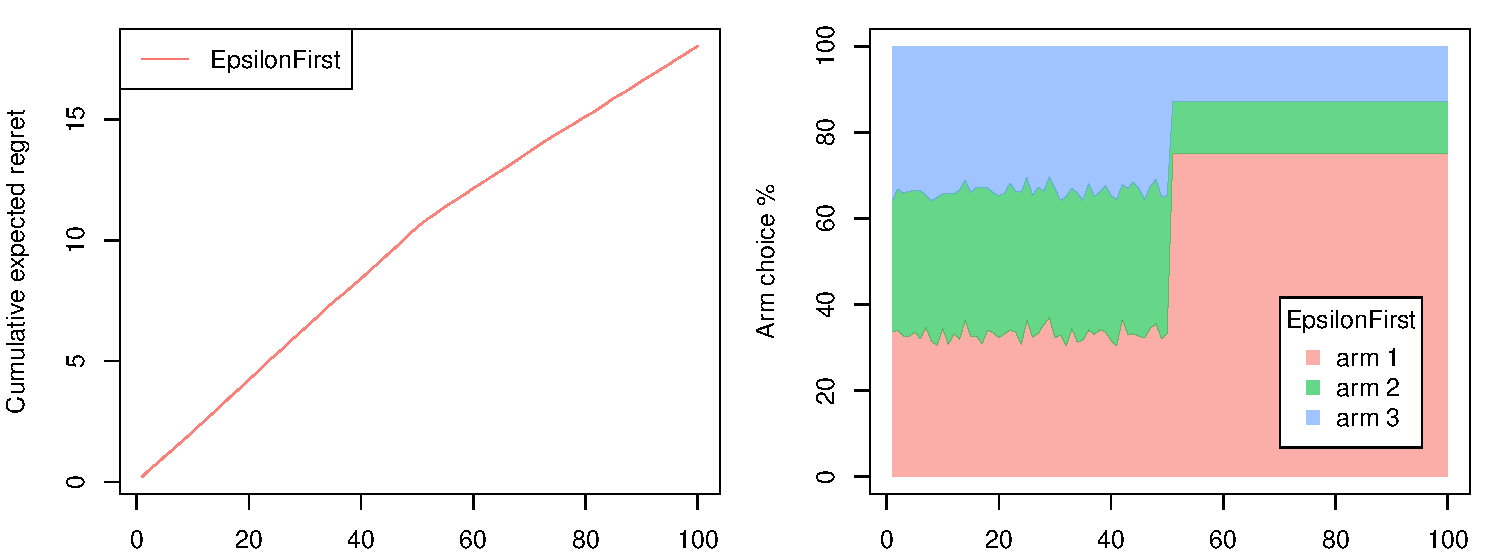
\includegraphics[width=\maxwidth,]{fig/efpolicy-1} \caption[Epsilon Greedy]{Epsilon Greedy}\label{fig:efpolicy}
\end{figure}


\end{knitrout}
\end{center}

\subsection{The Epsilon Greedy Policy}

Contrary to the previously introduced Epsilon First policy, an Epsilon Greedy algorithm does not divide exploitation and exploration into two strictly separate phases---it explores with a probability of $epsilon$ and exploits with a probability of $1-epsilon$, right from the start. That is, an Epsilon Greedy policy with an $epsilon$ of $0.1$ explores arms at random 10\% of the time. The other $1-epsilon$, or 90\% of the time, the policy "greedily" exploits the currently best-known arm.

This can be formalized in pseudocode as follows:

\begin{algorithm}[H]
\caption{Epsilon Greedy}
\label{Alg:EpsilonGreedy}
\begin{algorithmic}
\REQUIRE \(    \epsilon  \in \left[ 0,1 \right] \) - exploration tuning parameter
\STATE \( n_{a} \leftarrow 0 \) for all arms a \(  \in \left\{ 1, \dots, k \right\} \)  (count how many times an arm has been chosen)
\STATE \( \hat{\mu}_{a} \leftarrow 0 \) for all arms a  \(   \in \left\{ 1, \dots, k \right\} \)  (estimate of expected reward per arm)
% Run through time points:
\FOR{$t=1, \dots, T$}
	% Run through arms. Step 1, select which one to play
	\IF {sample from $\mathcal{N}(0,1) > \epsilon$}
		\STATE play arm \(a_t = \argmax_a  \hat{\mu}_{t-1,a}  \) with ties broken arbitrarily
	\ELSE
		\STATE play a random arm out of all arms a \(  \in \left\{ 1, \dots, k \right\} \)
	\ENDIF
	\STATE observe real-valued payoff $r_t$
	% Update:
	\STATE \( n_{a_{t}} \leftarrow n_{a_{t-1}} + 1  \)
   \STATE \( \hat{\mu}_{t,a_{t}} \leftarrow   \cfrac{r_t - \hat{\mu}_{t-1,a_{t}} }{n_{a_{t}}}   \)
\ENDFOR
\end{algorithmic}
\end{algorithm}

Converted to an EpsilonGreedyPolicy class:

\begin{knitrout}\small
\definecolor{shadecolor}{rgb}{0.969, 0.969, 0.969}\color{fgcolor}\begin{kframe}
\begin{alltt}
\hlstd{EpsilonGreedyPolicy} \hlkwb{<-} \hlstd{R6}\hlopt{::}\hlkwd{R6Class}\hlstd{(}
  \hlkwc{public} \hlstd{=} \hlkwd{list}\hlstd{(}
    \hlkwc{epsilon} \hlstd{=} \hlkwa{NULL}\hlstd{,}
    \hlkwc{initialize} \hlstd{=} \hlkwa{function}\hlstd{(}\hlkwc{epsilon} \hlstd{=} \hlnum{0.1}\hlstd{,} \hlkwc{name} \hlstd{=} \hlstr{"EGreedy"}\hlstd{) \{}
      \hlstd{super}\hlopt{$}\hlkwd{initialize}\hlstd{(name)}
      \hlstd{self}\hlopt{$}\hlstd{epsilon} \hlkwb{<-} \hlstd{epsilon}
    \hlstd{\},}
    \hlkwc{set_parameters} \hlstd{=} \hlkwa{function}\hlstd{() \{}
      \hlstd{self}\hlopt{$}\hlstd{theta_to_arms} \hlkwb{<-} \hlkwd{list}\hlstd{(}\hlstr{'n'} \hlstd{=} \hlnum{0}\hlstd{,} \hlstr{'mean'} \hlstd{=} \hlnum{0}\hlstd{)}
    \hlstd{\},}
    \hlkwc{get_action} \hlstd{=} \hlkwa{function}\hlstd{(}\hlkwc{context}\hlstd{,} \hlkwc{t}\hlstd{) \{}
      \hlkwa{if} \hlstd{(}\hlkwd{runif}\hlstd{(}\hlnum{1}\hlstd{)} \hlopt{>} \hlstd{epsilon) \{}
        \hlstd{action}\hlopt{$}\hlstd{choice} \hlkwb{<-} \hlkwd{max_in}\hlstd{(theta}\hlopt{$}\hlstd{mean)}
        \hlstd{action}\hlopt{$}\hlstd{propensity} \hlkwb{<-} \hlnum{1} \hlopt{-} \hlstd{self}\hlopt{$}\hlstd{epsilon}
      \hlstd{\}} \hlkwa{else} \hlstd{\{}
        \hlstd{action}\hlopt{$}\hlstd{choice} \hlkwb{<-} \hlkwd{sample.int}\hlstd{(context}\hlopt{$}\hlstd{k,} \hlnum{1}\hlstd{,} \hlkwc{replace} \hlstd{=} \hlnum{TRUE}\hlstd{)}
        \hlstd{action}\hlopt{$}\hlstd{propensity} \hlkwb{<-} \hlstd{epsilon}\hlopt{*}\hlstd{(}\hlnum{1}\hlopt{/}\hlstd{context}\hlopt{$}\hlstd{k)}
      \hlstd{\}}
      \hlstd{action}
    \hlstd{\},}
    \hlkwc{set_reward} \hlstd{=} \hlkwa{function}\hlstd{(}\hlkwc{context}\hlstd{,} \hlkwc{action}\hlstd{,} \hlkwc{reward}\hlstd{,} \hlkwc{t}\hlstd{) \{}
      \hlstd{arm} \hlkwb{<-} \hlstd{action}\hlopt{$}\hlstd{choice}
      \hlstd{reward} \hlkwb{<-} \hlstd{reward}\hlopt{$}\hlstd{reward}
      \hlkwd{inc}\hlstd{(theta}\hlopt{$}\hlstd{n[[arm]])}    \hlkwb{<-} \hlnum{1}
      \hlkwd{inc}\hlstd{(theta}\hlopt{$}\hlstd{mean[[arm]])} \hlkwb{<-} \hlstd{(reward} \hlopt{-} \hlstd{theta}\hlopt{$}\hlstd{mean[[arm]])} \hlopt{/} \hlstd{theta}\hlopt{$}\hlstd{n[[arm]]}
      \hlstd{theta}
    \hlstd{\}}
  \hlstd{)}
\hlstd{)}
\end{alltt}
\end{kframe}
\end{knitrout}

Assign the new class, together with \code{SyntheticBandit}, to an \code{Agent}. Again, assign the \code{Agent} to a \code{Simulator}. Then run the \code{Simulator} and \code{plot()}:

\begin{knitrout}\small
\definecolor{shadecolor}{rgb}{0.969, 0.969, 0.969}\color{fgcolor}\begin{kframe}
\begin{alltt}
\hlstd{horizon}            \hlkwb{<-} \hlnum{100}
\hlstd{simulations}        \hlkwb{<-} \hlnum{100}
\hlstd{weights}            \hlkwb{<-} \hlkwd{c}\hlstd{(}\hlnum{0.9}\hlstd{,} \hlnum{0.1}\hlstd{,} \hlnum{0.1}\hlstd{)}

\hlstd{policy}             \hlkwb{<-} \hlstd{EpsilonGreedyPolicy}\hlopt{$}\hlkwd{new}\hlstd{(}\hlkwc{epsilon} \hlstd{=} \hlnum{0.1}\hlstd{,} \hlkwc{name} \hlstd{=} \hlstr{"EG"}\hlstd{)}
\hlstd{bandit}             \hlkwb{<-} \hlstd{SyntheticBandit}\hlopt{$}\hlkwd{new}\hlstd{(}\hlkwc{weights} \hlstd{= weights)}

\hlstd{agent}              \hlkwb{<-} \hlstd{Agent}\hlopt{$}\hlkwd{new}\hlstd{(policy,bandit)}

\hlstd{simulator}          \hlkwb{<-} \hlstd{Simulator}\hlopt{$}\hlkwd{new}\hlstd{(}\hlkwc{agents} \hlstd{= agent,}
                                    \hlkwc{horizon} \hlstd{= horizon,}
                                    \hlkwc{simulations} \hlstd{= simulations,}
                                    \hlkwc{do_parallel} \hlstd{=} \hlnum{FALSE}\hlstd{)}

\hlstd{history}            \hlkwb{<-} \hlstd{simulator}\hlopt{$}\hlkwd{run}\hlstd{()}

\hlkwd{par}\hlstd{(}\hlkwc{mfrow} \hlstd{=} \hlkwd{c}\hlstd{(}\hlnum{1}\hlstd{,} \hlnum{2}\hlstd{),} \hlkwc{mar} \hlstd{=} \hlkwd{c}\hlstd{(}\hlnum{2}\hlstd{,}\hlnum{4}\hlstd{,}\hlnum{1}\hlstd{,}\hlnum{1}\hlstd{))}
\hlkwd{plot}\hlstd{(history,} \hlkwc{type} \hlstd{=} \hlstr{"cumulative"}\hlstd{,} \hlkwc{no_par} \hlstd{=} \hlnum{TRUE}\hlstd{)}
\hlkwd{plot}\hlstd{(history,} \hlkwc{type} \hlstd{=} \hlstr{"arms"}\hlstd{,} \hlkwc{no_par} \hlstd{=} \hlnum{TRUE}\hlstd{)}
\end{alltt}
\end{kframe}
\end{knitrout}
\begin{center}
\begin{knitrout}
\definecolor{shadecolor}{rgb}{0.969, 0.969, 0.969}\color{fgcolor}\begin{figure}[H]
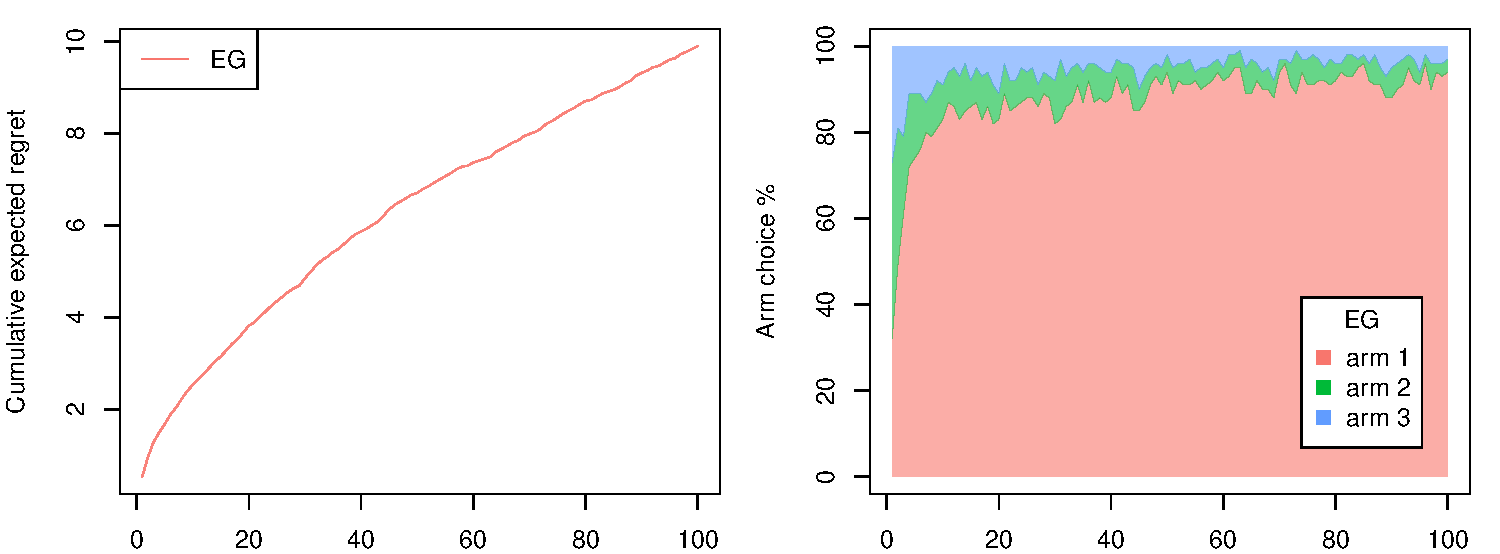
\includegraphics[width=\maxwidth,]{fig/egpolicy-1} \caption[Epsilon Greedy]{Epsilon Greedy}\label{fig:egpolicy}
\end{figure}


\end{knitrout}
\end{center}

\subsection{Contextual Bandit: LinUCB with Linear Disjoint Models}

As a final example of how to subclass \pkg{contextual}'s \code{Bandit} superclass, we move from non-contextual algorithms to a contextual one. As described in section 1, contextual bandits can make use of side information to help them choose the current best arm to play. For example, contextual information such as a website visitors' location may be related to which article's headline (or arm) on the frontpage of the website will be clicked on most.

Here, we show how to implement and evaluate probably one of the most cited out of all contextual policies, the LinUCB algorithm with Linear Disjoint Models. The policy is more complicated than the previous two bandits, but when following its pseudocode description to the letter, it translates nicely to yet another Bandit subclass.

The LinUCBDisjoint algorithm works by running a linear regression with coefficients for each of \code{d} contextual features on the available historical data. Then the algorithm observes the new context and uses this context to generate a predicted reward based on the regression model. Importantly, the algorithm also generates a confidence interval for the predicted payoff for each of \code{k} arms. The policy then chooses the arm with the highest upper confidence bound. In pseudocode:

\begin{algorithm}[H]
\caption{LinUCB with linear disjoint models}
\label{Alg:LinUCBDisjoint}
\begin{algorithmic}
\REQUIRE $\alpha$ \(  \in \mathbb{R}^{+} \), exploration tuning parameter
% Run through time points:
\FOR{$t=1, \dots, T$}
          \STATE Observe features of all arms \(  a \in \mathcal{A}_{t}: x_{t,a} \in \mathbb{R}^{d}\)
	% Run through arms. Step 1, select which one to play
	\FOR{ \(  a \in \mathcal{A}_{t}\)}
	          \IF{\(a\) is new}
		      \STATE \(A_{a} \leftarrow I_{d}  \)  (d-dimensional identity matrix)
		      \STATE \(b_{a} \leftarrow 0_{d\times1}   \) (d-dimensional zero vector)
		\ENDIF
		\STATE \( \hat{\theta}_{a} \leftarrow A_{a}^{-1}b_{a} \)
		\STATE \( p_{t,a} \leftarrow \hat{\theta}_{a}^{T} + \alpha  \sqrt{ x_{t,a}^{T} A_{a}^{-1}x_{t,a}} \)
	\ENDFOR
	% allocate to arm
	\STATE Play arm \(a_t = \argmax_a  p_{t,a}  \) with ties broken arbitrarily and observe real-valued payoff $r_t$
	% Update:
           \STATE \( A_{a_{t}} \leftarrow A_{a_{t}}+ x_{t,a_{t}}x_{t,a_{t}}^{T} \)
           \STATE  \( b_{a_{t}} \leftarrow b_{a_{t}}+ r_{t}x_{t,a_{t}}  \)
\ENDFOR
\end{algorithmic}
\end{algorithm}

Next, translating the above pseudocode into a well organized \code{Bandit} subclass:

\begin{knitrout}\small
\definecolor{shadecolor}{rgb}{0.969, 0.969, 0.969}\color{fgcolor}\begin{kframe}
\begin{alltt}
\hlcom{#' @export}
\hlstd{LinUCBDisjointPolicy} \hlkwb{<-} \hlstd{R6}\hlopt{::}\hlkwd{R6Class}\hlstd{(}
  \hlkwc{public} \hlstd{=} \hlkwd{list}\hlstd{(}
    \hlkwc{alpha} \hlstd{=} \hlkwa{NULL}\hlstd{,}
    \hlkwc{initialize} \hlstd{=} \hlkwa{function}\hlstd{(}\hlkwc{alpha} \hlstd{=} \hlnum{1.0}\hlstd{,} \hlkwc{name} \hlstd{=} \hlstr{"LinUCBDisjoint"}\hlstd{) \{}
      \hlstd{super}\hlopt{$}\hlkwd{initialize}\hlstd{(name)}
      \hlstd{self}\hlopt{$}\hlstd{alpha} \hlkwb{<-} \hlstd{alpha}
    \hlstd{\},}
    \hlkwc{set_parameters} \hlstd{=} \hlkwa{function}\hlstd{() \{}
      \hlstd{self}\hlopt{$}\hlstd{theta_to_arms} \hlkwb{<-} \hlkwd{list}\hlstd{(} \hlstr{'A'} \hlstd{=} \hlkwd{diag}\hlstd{(}\hlnum{1}\hlstd{,self}\hlopt{$}\hlstd{d,self}\hlopt{$}\hlstd{d),} \hlstr{'b'} \hlstd{=} \hlkwd{rep}\hlstd{(}\hlnum{0}\hlstd{,self}\hlopt{$}\hlstd{d))}
    \hlstd{\},}
    \hlkwc{get_action} \hlstd{=} \hlkwa{function}\hlstd{(}\hlkwc{context}\hlstd{,} \hlkwc{t}\hlstd{) \{}
      \hlstd{expected_rewards} \hlkwb{<-} \hlkwd{rep}\hlstd{(}\hlnum{0.0}\hlstd{, context}\hlopt{$}\hlstd{k)}
      \hlkwa{for} \hlstd{(arm} \hlkwa{in} \hlnum{1}\hlopt{:}\hlstd{self}\hlopt{$}\hlstd{k) \{}
        \hlstd{X}          \hlkwb{<-}  \hlstd{context}\hlopt{$}\hlstd{X[,arm]}
        \hlstd{A}          \hlkwb{<-}  \hlstd{theta}\hlopt{$}\hlstd{A[[arm]]}
        \hlstd{b}          \hlkwb{<-}  \hlstd{theta}\hlopt{$}\hlstd{b[[arm]]}
        \hlstd{A_inv}      \hlkwb{<-}  \hlkwd{solve}\hlstd{(A)}

        \hlstd{theta_hat}  \hlkwb{<-}  \hlstd{A_inv} \hlopt \hlstd{b}
        \hlstd{mean}       \hlkwb{<-}  \hlstd{X} \hlopt \hlstd{theta_hat}
        \hlstd{sd}         \hlkwb{<-}  \hlkwd{sqrt}\hlstd{(}\hlkwd{tcrossprod}\hlstd{(X} \hlopt \hlstd{A_inv, X))}
        \hlstd{expected_rewards[arm]} \hlkwb{<-} \hlstd{mean} \hlopt{+} \hlstd{alpha} \hlopt{*} \hlstd{sd}
      \hlstd{\}}
      \hlstd{action}\hlopt{$}\hlstd{choice}  \hlkwb{<-} \hlkwd{max_in}\hlstd{(expected_rewards)}
      \hlstd{action}
    \hlstd{\},}
    \hlkwc{set_reward} \hlstd{=} \hlkwa{function}\hlstd{(}\hlkwc{context}\hlstd{,} \hlkwc{action}\hlstd{,} \hlkwc{reward}\hlstd{,} \hlkwc{t}\hlstd{) \{}
      \hlstd{arm} \hlkwb{<-} \hlstd{action}\hlopt{$}\hlstd{choice}
      \hlstd{reward} \hlkwb{<-} \hlstd{reward}\hlopt{$}\hlstd{reward}
      \hlstd{Xa} \hlkwb{<-} \hlstd{context}\hlopt{$}\hlstd{X[,arm]}

      \hlkwd{inc}\hlstd{(theta}\hlopt{$}\hlstd{A[[arm]])} \hlkwb{<-} \hlkwd{outer}\hlstd{(Xa, Xa)}
      \hlkwd{inc}\hlstd{(theta}\hlopt{$}\hlstd{b[[arm]])} \hlkwb{<-} \hlstd{reward} \hlopt{*} \hlstd{Xa}

      \hlstd{theta}
    \hlstd{\}}
  \hlstd{)}
\hlstd{)}
\end{alltt}
\end{kframe}
\end{knitrout}

Now it is possible to evaluate the \code{LinUCBDisjointPolicy} using a Bernoulli \code{SyntheticBandit} with three arms and three context features. In the code below we define each of \code{SyntheticBandit}'s arms to be, on average, equally probable to return a reward. However, at the same time, the presence of a random context feature vector exercises a strong influence on the distribution of rewards over the arms per time step t: in the presence of a specific feature, one of the arms becomes much more likely to offer a reward. In this setting, the \code{EpsilonGreedyPolicy} does not do better than chance. But the \code{LinUCBDisjointPolicy} is able to learn the relationships between arms, rewards, and features without much difficulty:

\begin{knitrout}\small
\definecolor{shadecolor}{rgb}{0.969, 0.969, 0.969}\color{fgcolor}\begin{kframe}
\begin{alltt}
\hlstd{horizon}      \hlkwb{<-} \hlnum{100L}
\hlstd{simulations}  \hlkwb{<-} \hlnum{300L}

                      \hlcom{# k=1  k=2  k=3              -> columns represent arms}

\hlstd{weights}     \hlkwb{<-} \hlkwd{matrix}\hlstd{(}\hlkwd{c}\hlstd{(}\hlnum{0.8}\hlstd{,} \hlnum{0.1}\hlstd{,} \hlnum{0.1}\hlstd{,}     \hlcom{# d=1   -> rows represent}
                        \hlnum{0.1}\hlstd{,} \hlnum{0.8}\hlstd{,} \hlnum{0.1}\hlstd{,}     \hlcom{# d=2      context features}
                        \hlnum{0.1}\hlstd{,} \hlnum{0.1}\hlstd{,} \hlnum{0.8}\hlstd{),}    \hlcom{# d=3}

                        \hlkwc{nrow} \hlstd{=} \hlnum{3}\hlstd{,} \hlkwc{ncol} \hlstd{=} \hlnum{3}\hlstd{,} \hlkwc{byrow} \hlstd{=} \hlnum{TRUE}\hlstd{)}

\hlstd{bandit}      \hlkwb{<-} \hlstd{SyntheticBandit}\hlopt{$}\hlkwd{new}\hlstd{(}\hlkwc{weights} \hlstd{= weights,} \hlkwc{precaching} \hlstd{=} \hlnum{TRUE}\hlstd{)}

\hlstd{agents}      \hlkwb{<-} \hlkwd{list}\hlstd{(Agent}\hlopt{$}\hlkwd{new}\hlstd{(EpsilonGreedyPolicy}\hlopt{$}\hlkwd{new}\hlstd{(}\hlnum{0.1}\hlstd{,} \hlstr{"EGreedy"}\hlstd{), bandit),}
                    \hlstd{Agent}\hlopt{$}\hlkwd{new}\hlstd{(LinUCBDisjointPolicy}\hlopt{$}\hlkwd{new}\hlstd{(}\hlnum{1.0}\hlstd{,} \hlstr{"LinUCB"}\hlstd{), bandit))}

\hlstd{simulation}  \hlkwb{<-} \hlstd{Simulator}\hlopt{$}\hlkwd{new}\hlstd{(agents, horizon, simulations,} \hlkwc{do_parallel} \hlstd{=} \hlnum{FALSE}\hlstd{)}
\hlstd{history}     \hlkwb{<-} \hlstd{simulation}\hlopt{$}\hlkwd{run}\hlstd{()}

\hlkwd{par}\hlstd{(}\hlkwc{mfrow} \hlstd{=} \hlkwd{c}\hlstd{(}\hlnum{1}\hlstd{,} \hlnum{2}\hlstd{),} \hlkwc{mar} \hlstd{=} \hlkwd{c}\hlstd{(}\hlnum{2}\hlstd{,}\hlnum{4}\hlstd{,}\hlnum{1}\hlstd{,}\hlnum{1}\hlstd{))}
\hlkwd{plot}\hlstd{(history,} \hlkwc{type} \hlstd{=} \hlstr{"cumulative"}\hlstd{,} \hlkwc{regret} \hlstd{=} \hlnum{FALSE}\hlstd{,} \hlkwc{no_par} \hlstd{=} \hlnum{TRUE}\hlstd{)}
\hlkwd{plot}\hlstd{(history,} \hlkwc{type} \hlstd{=} \hlstr{"cumulative"}\hlstd{,} \hlkwc{no_par} \hlstd{=} \hlnum{TRUE}\hlstd{)}
\end{alltt}
\end{kframe}
\end{knitrout}
\begin{center}
\begin{knitrout}
\definecolor{shadecolor}{rgb}{0.969, 0.969, 0.969}\color{fgcolor}\begin{figure}[H]
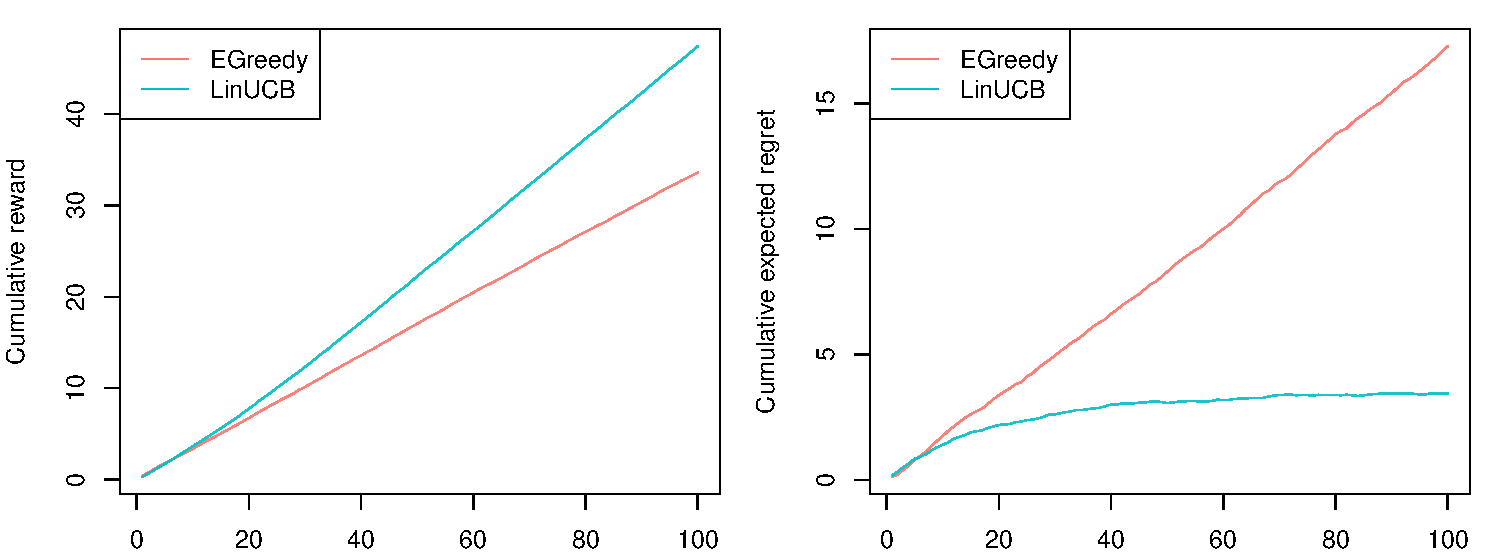
\includegraphics[width=\maxwidth,]{fig/lucbpolicy-1} \caption[The contextual LinUCB algorithm with linear disjoint models, following Li et al]{The contextual LinUCB algorithm with linear disjoint models, following Li et al. (2010), compared to a non-contextual basic EpsilonGreedy policy tested on data generated by a contextual synthetic Bandit for two performance measures: left cumulative reward, right expected cumulative regret. }\label{fig:lucbpolicy}
\end{figure}


\end{knitrout}
\end{center}

\subsection{Subclassing Policies and Bandits}

\pkg{contextual}'s extensibility does, of course, not limit itself to the subclassing of \code{Policy} classes. Through its R6 based object system it is easy to extend and override any \pkg{contextual} super- or subclass. Below, we demonstrate how to apply that extensibility to sub-subclass one Bandit and one Policy subclass.
First, we extend \code{ BasicBandit}'s code{PoissonRewardBandit}, replacing \code{ BasicBandit}'s Bernoulli based reward function with a Poisson based one. Next, we implement an \code{EpsilonGreedyAnnealingPolicy} version of the Epsilon Greedy policy introduced in section 4.2---where its \code{EpsilonGreedyAnnealingPolicy} subclass introduces a gradual reduction ("annealing") of the policy's $epsilon$ parameter over T, in effect moving the policy from more explorative to a more exploitative over time.

\begin{knitrout}\small
\definecolor{shadecolor}{rgb}{0.969, 0.969, 0.969}\color{fgcolor}\begin{kframe}
\begin{alltt}
\hlstd{PoissonRewardBandit} \hlkwb{<-} \hlstd{R6}\hlopt{::}\hlkwd{R6Class}\hlstd{(}
  \hlstr{"PoissonRewardBandit"}\hlstd{,}
  \hlcom{# Class extends BasicBandit}
  \hlkwc{inherit} \hlstd{= BasicBandit,}
  \hlkwc{public} \hlstd{=} \hlkwd{list}\hlstd{(}
    \hlkwc{initialize} \hlstd{=} \hlkwa{function}\hlstd{(}\hlkwc{weights}\hlstd{) \{}
      \hlstd{super}\hlopt{$}\hlkwd{initialize}\hlstd{(weights)}
    \hlstd{\},}
    \hlcom{# Overrides BasicBandit's get_reward to generate Poisson based rewards}
    \hlkwc{get_reward} \hlstd{=} \hlkwa{function}\hlstd{(}\hlkwc{t}\hlstd{,} \hlkwc{context}\hlstd{,} \hlkwc{action}\hlstd{) \{}
      \hlstd{reward_means} \hlkwb{=} \hlkwd{c}\hlstd{(}\hlnum{2}\hlstd{,}\hlnum{2}\hlstd{,}\hlnum{2}\hlstd{)}
      \hlstd{rpm} \hlkwb{<-} \hlkwd{rpois}\hlstd{(}\hlnum{3}\hlstd{, reward_means)}
      \hlstd{private}\hlopt{$}\hlstd{R} \hlkwb{<-} \hlkwd{matrix}\hlstd{(rpm} \hlopt{<} \hlstd{self}\hlopt{$}\hlkwd{get_weights}\hlstd{(), self}\hlopt{$}\hlstd{k, self}\hlopt{$}\hlstd{d)}\hlopt{*}\hlnum{1}
      \hlkwd{list}\hlstd{(}
        \hlkwc{reward}                   \hlstd{= private}\hlopt{$}\hlstd{R[action}\hlopt{$}\hlstd{choice],}
        \hlkwc{optimal_reward_value}     \hlstd{= private}\hlopt{$}\hlstd{R[}\hlkwd{which.max}\hlstd{(private}\hlopt{$}\hlstd{R)]}
      \hlstd{)}
    \hlstd{\}}
  \hlstd{)}
\hlstd{)}
\hlstd{EpsilonGreedyAnnealingPolicy} \hlkwb{<-} \hlstd{R6}\hlopt{::}\hlkwd{R6Class}\hlstd{(}
  \hlstr{"EpsilonGreedyAnnealingPolicy"}\hlstd{,}
  \hlcom{# Class extends EpsilonGreedyPolicy}
  \hlkwc{inherit} \hlstd{= EpsilonGreedyPolicy,}
  \hlkwc{portable} \hlstd{=} \hlnum{FALSE}\hlstd{,}
  \hlkwc{public} \hlstd{=} \hlkwd{list}\hlstd{(}
    \hlcom{# Override EpsilonGreedyPolicy's get_action, use annealing epsilon}
    \hlkwc{get_action} \hlstd{=} \hlkwa{function}\hlstd{(}\hlkwc{t}\hlstd{,} \hlkwc{context}\hlstd{) \{}
      \hlstd{self}\hlopt{$}\hlstd{epsilon} \hlkwb{<-} \hlnum{1} \hlopt{/} \hlkwd{log}\hlstd{(t} \hlopt{+} \hlnum{0.0000001}\hlstd{)}
      \hlstd{super}\hlopt{$}\hlkwd{get_action}\hlstd{(t, context)}
    \hlstd{\}}
  \hlstd{)}
\hlstd{)}
\hlstd{weights}     \hlkwb{<-} \hlkwd{c}\hlstd{(}\hlnum{7}\hlstd{,}\hlnum{1}\hlstd{,}\hlnum{2}\hlstd{)}
\hlstd{horizon}     \hlkwb{<-} \hlnum{200}
\hlstd{simulations} \hlkwb{<-} \hlnum{100}
\hlstd{bandit}      \hlkwb{<-} \hlstd{PoissonRewardBandit}\hlopt{$}\hlkwd{new}\hlstd{(weights)}
\hlstd{agents}      \hlkwb{<-} \hlkwd{list}\hlstd{(Agent}\hlopt{$}\hlkwd{new}\hlstd{(EpsilonGreedyPolicy}\hlopt{$}\hlkwd{new}\hlstd{(}\hlnum{0.1}\hlstd{,} \hlstr{"EG Annealing"}\hlstd{), bandit),}
                    \hlstd{Agent}\hlopt{$}\hlkwd{new}\hlstd{(EpsilonGreedyAnnealingPolicy}\hlopt{$}\hlkwd{new}\hlstd{(}\hlnum{0.1}\hlstd{,} \hlstr{"EG"}\hlstd{), bandit))}
\hlstd{simulation}  \hlkwb{<-} \hlstd{Simulator}\hlopt{$}\hlkwd{new}\hlstd{(agents, horizon, simulations,} \hlkwc{do_parallel} \hlstd{=} \hlnum{FALSE}\hlstd{)}

\hlstd{history}     \hlkwb{<-} \hlstd{simulation}\hlopt{$}\hlkwd{run}\hlstd{()}

\hlkwd{par}\hlstd{(}\hlkwc{mfrow} \hlstd{=} \hlkwd{c}\hlstd{(}\hlnum{1}\hlstd{,} \hlnum{2}\hlstd{),} \hlkwc{mar} \hlstd{=} \hlkwd{c}\hlstd{(}\hlnum{2}\hlstd{,}\hlnum{4}\hlstd{,}\hlnum{1}\hlstd{,}\hlnum{1}\hlstd{))}
\hlkwd{plot}\hlstd{(history,} \hlkwc{type} \hlstd{=} \hlstr{"cumulative"}\hlstd{,} \hlkwc{no_par} \hlstd{=} \hlnum{TRUE}\hlstd{)}
\hlkwd{plot}\hlstd{(history,} \hlkwc{type} \hlstd{=} \hlstr{"average"}\hlstd{,} \hlkwc{regret} \hlstd{=} \hlnum{FALSE}\hlstd{,} \hlkwc{no_par} \hlstd{=} \hlnum{TRUE}\hlstd{)}
\end{alltt}
\end{kframe}
\end{knitrout}
\begin{center}
\begin{knitrout}
\definecolor{shadecolor}{rgb}{0.969, 0.969, 0.969}\color{fgcolor}\begin{figure}[H]
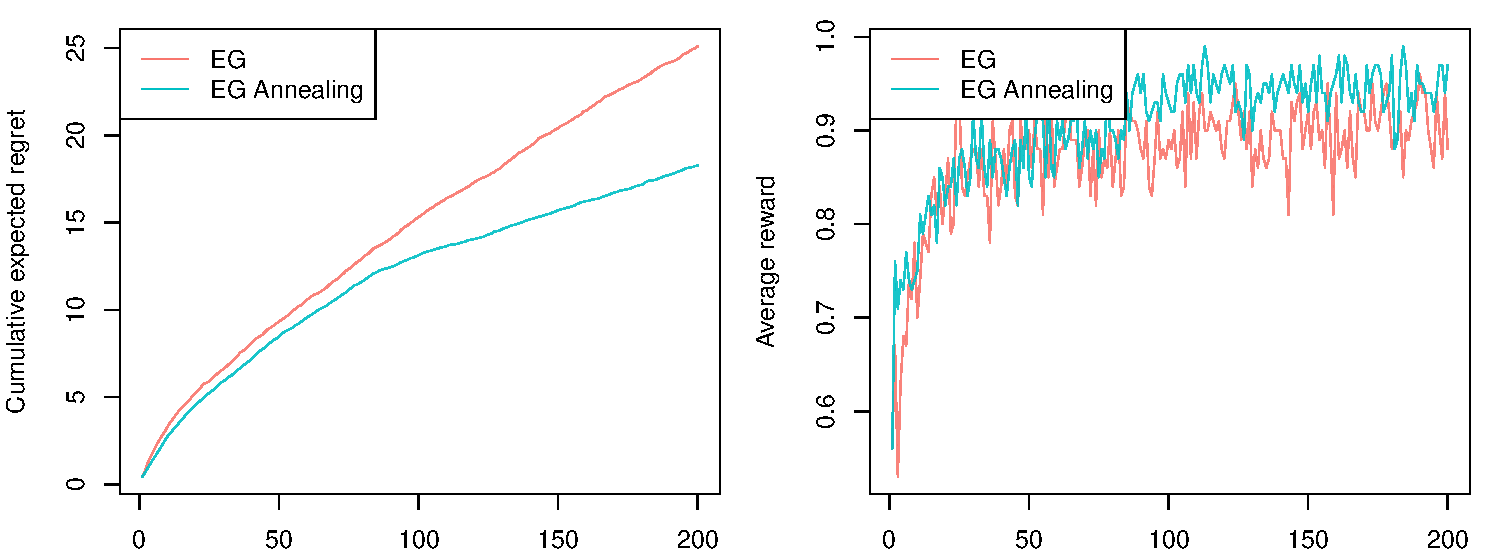
\includegraphics[width=\maxwidth,]{fig/poissonplot-1} \caption[Extending BasicBandit and EpsilonGreedyPolicy]{Extending BasicBandit and EpsilonGreedyPolicy}\label{fig:poissonplot}
\end{figure}


\end{knitrout}
\end{center}

\section{Offline evaluation}

Though it is, as demonstrated in the previous section, relatively easy to create basic synthetic Bandits to test simple MAB and cMAB policies, the creation of more elaborate simulations that generate more complex contexts for more demanding policies can become very complicated very fast. So much so, that the implementation of such simulators regularly becomes more intricate than the analysis and implementation of the policies themselves. Moreover, even when succeeding in surpassing these technical challenges, it remains an open question if an evaluation based on simulated data reflects real-world applications since modeling by definition introduces bias.

It would, of course, be possible to evaluate policies by running them in a live setting. Such live evaluations would undoubtedly deliver unbiased, realistic estimates of a policy's effectiveness. However, the use of live data makes it more difficult to compare multiple policies at the same, as it is not possible to test multiple policies at the same time with the same user. Using live data is usually also much slower than an offline evaluation, as online evaluations are dependent on active user interventions. Furthermore, the testing of policies on a live target audience, such as patients or customers, with potentially suboptimal policies, could become either dangerous or very expensive.

Another unbiased approach to testing MAB and cMAB policies would be to make use of offline historical data or logs. Such a data source does need to contain observed contexts and rewards, and any actions or arms must have been selected either at random or with a known probability per arm \( D = (p_1,p_2,p_3,...,p_k) \). That is, such data sets contain at least \( D = (x_{t,a_t},a_{t},r_{t,a_t}) \), or, in the case of know probabilities per arm \( D = (x_{t,a_t},a_{t},r_{t,a_t},p_a) \). Not only does such offline data pre-empt the issues of bias and model complexity, but it also offers the advantage that such data is widely available, as historical logs, as benchmark data sets for supervised learning, and more.

There is a catch though; when we make use of offline data, we miss out on user feedback every time a policy under evaluation suggests a different arm from the one that was initially selected and saved to the offline data set. In other words, offline data is "partially labeled" in respect to evaluated Bandit policies. However, as shown in the following subsections, it is possible to get around this partial labeling problem by discarding part of the data, and by making the most of any additional information in offline data sets.

\subsection{Offline Evaluation of Policies through LiSamplingBandit}

The first, and most important, step in using offline data in policy evaluation is to recognize that we need to limit our evaluation to those rows of data where the arm selected is the same as the one that is suggested by the policy under evaluation. In pseudocode:

\begin{algorithm}[H]
\caption{Li Policy Evaluator}
\label{Alg:LiBandit}
\begin{algorithmic}
\REQUIRE  Policy $\piup$ \\
                 Data stream of events $S$ of length $T$  \\
                 $h_0 \leftarrow \emptyset$ {An initially empty history log}\\
                 $R_\pi \leftarrow 0$ {An initially zero total cumulative reward}\\
                 $L \leftarrow 0$ {An initially zero length counter of valid events}
% Run through time points:
\FOR{$t=1, \dots, T$}
	\STATE Get the $t$-th event \( (x_{t,a_t},a_{t},r_{t,a_t}) \) from  $S$
	\IF {\(\pi \left( h_{t-1},x_{t,a_t} \right) = a_t\)}
	       \STATE $h_{t} \leftarrow $  \(\textrm{CONCATENATE}\left( h_{t-1},(x_{t,a_t},a_{t},r_{t,a_t})  \right)\)
	       \STATE $R_\pi = R_\pi + r_{t,a_t}$
	       \STATE $L = L + 1$
	\ELSE
	        \STATE $h_{t} \leftarrow  h_{t-1} $
	\ENDIF
\ENDFOR
\STATE Output: rate of cumulative regret $R_\pi / L $
\end{algorithmic}
\end{algorithm}

Converted to a contextual BasicBandit subclass and run on a large data set:

\begin{knitrout}\small
\definecolor{shadecolor}{rgb}{0.969, 0.969, 0.969}\color{fgcolor}\begin{kframe}
\begin{alltt}
\hlstd{BasicLiBandit} \hlkwb{<-} \hlstd{R6}\hlopt{::}\hlkwd{R6Class}\hlstd{(}
  \hlstr{"BasicLiBandit"}\hlstd{,}
  \hlkwc{inherit} \hlstd{= BasicBandit,}
  \hlkwc{portable} \hlstd{=} \hlnum{TRUE}\hlstd{,}
  \hlkwc{class} \hlstd{=} \hlnum{FALSE}\hlstd{,}
  \hlkwc{private} \hlstd{=} \hlkwd{list}\hlstd{(}
    \hlkwc{S} \hlstd{=} \hlkwa{NULL}
  \hlstd{),}
  \hlkwc{public} \hlstd{=} \hlkwd{list}\hlstd{(}
    \hlkwc{initialize}   \hlstd{=} \hlkwa{function}\hlstd{(}\hlkwc{data_stream}\hlstd{,} \hlkwc{arms}\hlstd{) \{}
      \hlstd{self}\hlopt{$}\hlstd{k} \hlkwb{<-} \hlstd{arms}
      \hlstd{self}\hlopt{$}\hlstd{d} \hlkwb{<-} \hlnum{1}
      \hlstd{private}\hlopt{$}\hlstd{S} \hlkwb{<-} \hlstd{data_stream}
    \hlstd{\},}
    \hlkwc{get_context} \hlstd{=} \hlkwa{function}\hlstd{(}\hlkwc{index}\hlstd{) \{}
      \hlstd{contextlist} \hlkwb{<-} \hlkwd{list}\hlstd{(}
        \hlkwc{k} \hlstd{= self}\hlopt{$}\hlstd{k,}
        \hlkwc{d} \hlstd{= self}\hlopt{$}\hlstd{d,}
        \hlkwc{X} \hlstd{=} \hlkwd{matrix}\hlstd{(}\hlnum{1}\hlstd{,self}\hlopt{$}\hlstd{d,self}\hlopt{$}\hlstd{k)} \hlcom{# no context}
      \hlstd{)}
      \hlstd{contextlist}
    \hlstd{\},}
    \hlkwc{get_reward} \hlstd{=} \hlkwa{function}\hlstd{(}\hlkwc{index}\hlstd{,} \hlkwc{context}\hlstd{,} \hlkwc{action}\hlstd{) \{}
      \hlstd{reward_at_index} \hlkwb{<-} \hlkwd{as.double}\hlstd{(private}\hlopt{$}\hlstd{S}\hlopt{$}\hlstd{reward[[index]])}
      \hlkwa{if} \hlstd{(private}\hlopt{$}\hlstd{S}\hlopt{$}\hlstd{choice[[index]]} \hlopt{==} \hlstd{action}\hlopt{$}\hlstd{choice) \{}
        \hlkwd{list}\hlstd{(}\hlkwc{reward} \hlstd{= reward_at_index)}
      \hlstd{\}} \hlkwa{else} \hlstd{\{}
        \hlkwa{NULL}
      \hlstd{\}}
    \hlstd{\}}
  \hlstd{)}
\hlstd{)}

\hlkwd{library}\hlstd{(data.table)}
\hlkwd{library}\hlstd{(RCurl)}
\hlkwd{library}\hlstd{(foreign)}

\hlstd{url} \hlkwb{<-} \hlstr{"https://raw.githubusercontent.com/Nth-iteration-labs/"}
\hlstd{url} \hlkwb{<-} \hlkwd{paste0}\hlstd{(url,}\hlstr{"contextual_data/master/PersuasionAPI/persuasion.csv"}\hlstd{)}

\hlstd{website_data}   \hlkwb{<-} \hlkwd{getURL}\hlstd{(url)}
\hlstd{website_data}   \hlkwb{<-} \hlkwd{setDT}\hlstd{(}\hlkwd{read.csv}\hlstd{(}\hlkwd{textConnection}\hlstd{(persuasion_data)))}
\hlstd{horizon}        \hlkwb{<-} \hlnum{350000L}
\hlstd{simulations}    \hlkwb{<-} \hlnum{100L}
\hlstd{bandit}         \hlkwb{<-} \hlstd{BasicLiBandit}\hlopt{$}\hlkwd{new}\hlstd{(website_data,} \hlkwc{arms} \hlstd{=} \hlnum{4}\hlstd{)}
\hlstd{agent}          \hlkwb{<-} \hlstd{Agent}\hlopt{$}\hlkwd{new}\hlstd{(UCB1Policy}\hlopt{$}\hlkwd{new}\hlstd{(), bandit)}
\hlstd{history}        \hlkwb{<-} \hlstd{Simulator}\hlopt{$}\hlkwd{new}\hlstd{(agent, horizon, simulations,} \hlkwc{reindex_t} \hlstd{=} \hlnum{TRUE}\hlstd{)}\hlopt{$}\hlkwd{run}\hlstd{()}

\hlkwd{par}\hlstd{(}\hlkwc{mfrow} \hlstd{=} \hlkwd{c}\hlstd{(}\hlnum{1}\hlstd{,} \hlnum{2}\hlstd{),} \hlkwc{mar} \hlstd{=} \hlkwd{c}\hlstd{(}\hlnum{2}\hlstd{,}\hlnum{4}\hlstd{,}\hlnum{1}\hlstd{,}\hlnum{1}\hlstd{))}
\hlkwd{plot}\hlstd{(history,} \hlkwc{type} \hlstd{=} \hlstr{"cumulative"}\hlstd{,} \hlkwc{regret} \hlstd{=} \hlnum{FALSE}\hlstd{,}
     \hlkwc{rate} \hlstd{=} \hlnum{TRUE}\hlstd{,} \hlkwc{ylim} \hlstd{=} \hlkwd{c}\hlstd{(}\hlnum{0.0105}\hlstd{,} \hlnum{0.015}\hlstd{))}
\end{alltt}
\end{kframe}
\end{knitrout}

\begin{figure}[H]
  \centering
    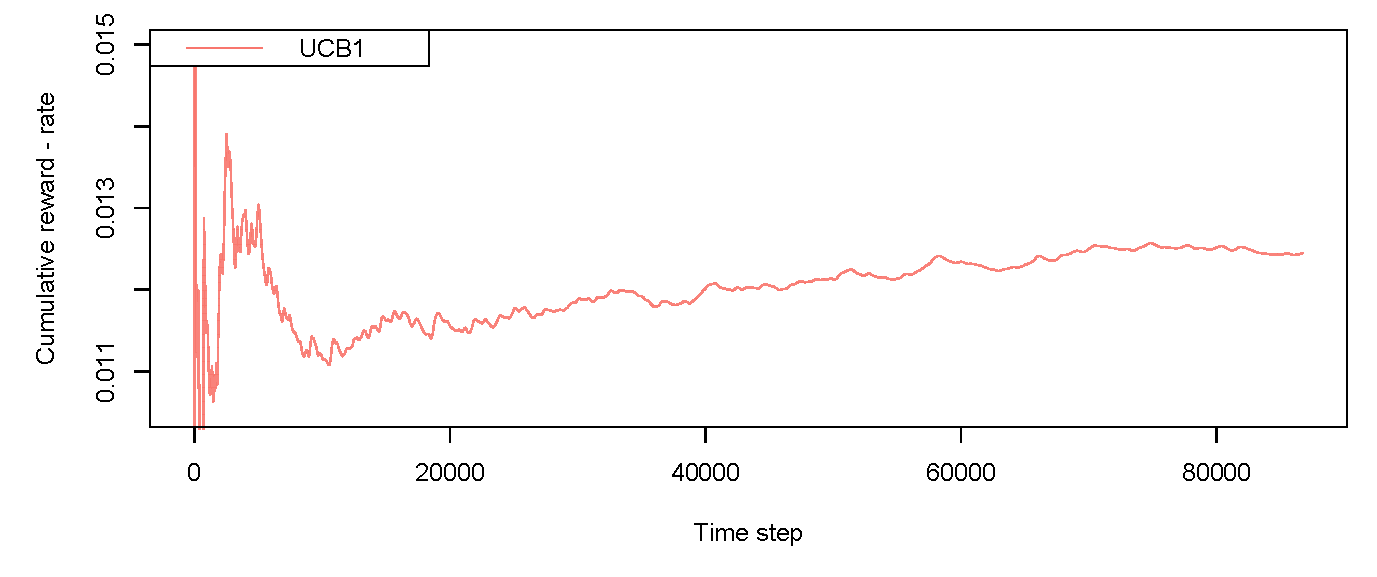
\includegraphics[width=.99\textwidth]{fig/ucb_offline}
    \label{fig:ucb_offline}
      \caption{An UCB1 policy evaluated on a Li Bandit. The Bandit samples from 350000 rows with clicks for rewards and the display of one of four “persuasive strategies” to users of an online store representing the offline Bandit's four arms.}
\end{figure}

\subsubsection{Offline evaluation through DoublyRobustBandit}

*** insert algorithm ***
*** insert code ***

\section{Replication of existing studies}

Here replication with yahoo dataset

\section{Parallelization}

\subsubsection{General}

Parallel is great!

\subsubsection{Amazon EC2}

Amazon EC2 rocks.

\subsubsection{Microsoft Azure}

Azure is cool too.

\subsubsection{Tradeoffs}

Time is of the essence...

\section{Extra greedy UCB}

Now with extra greedy!

And lock in feedback too? And dueling? and..

\section{Conclusion}
\label{sec:conc4}

\section{UML Diagrams}

\begin{figure}[H]
  \centering
    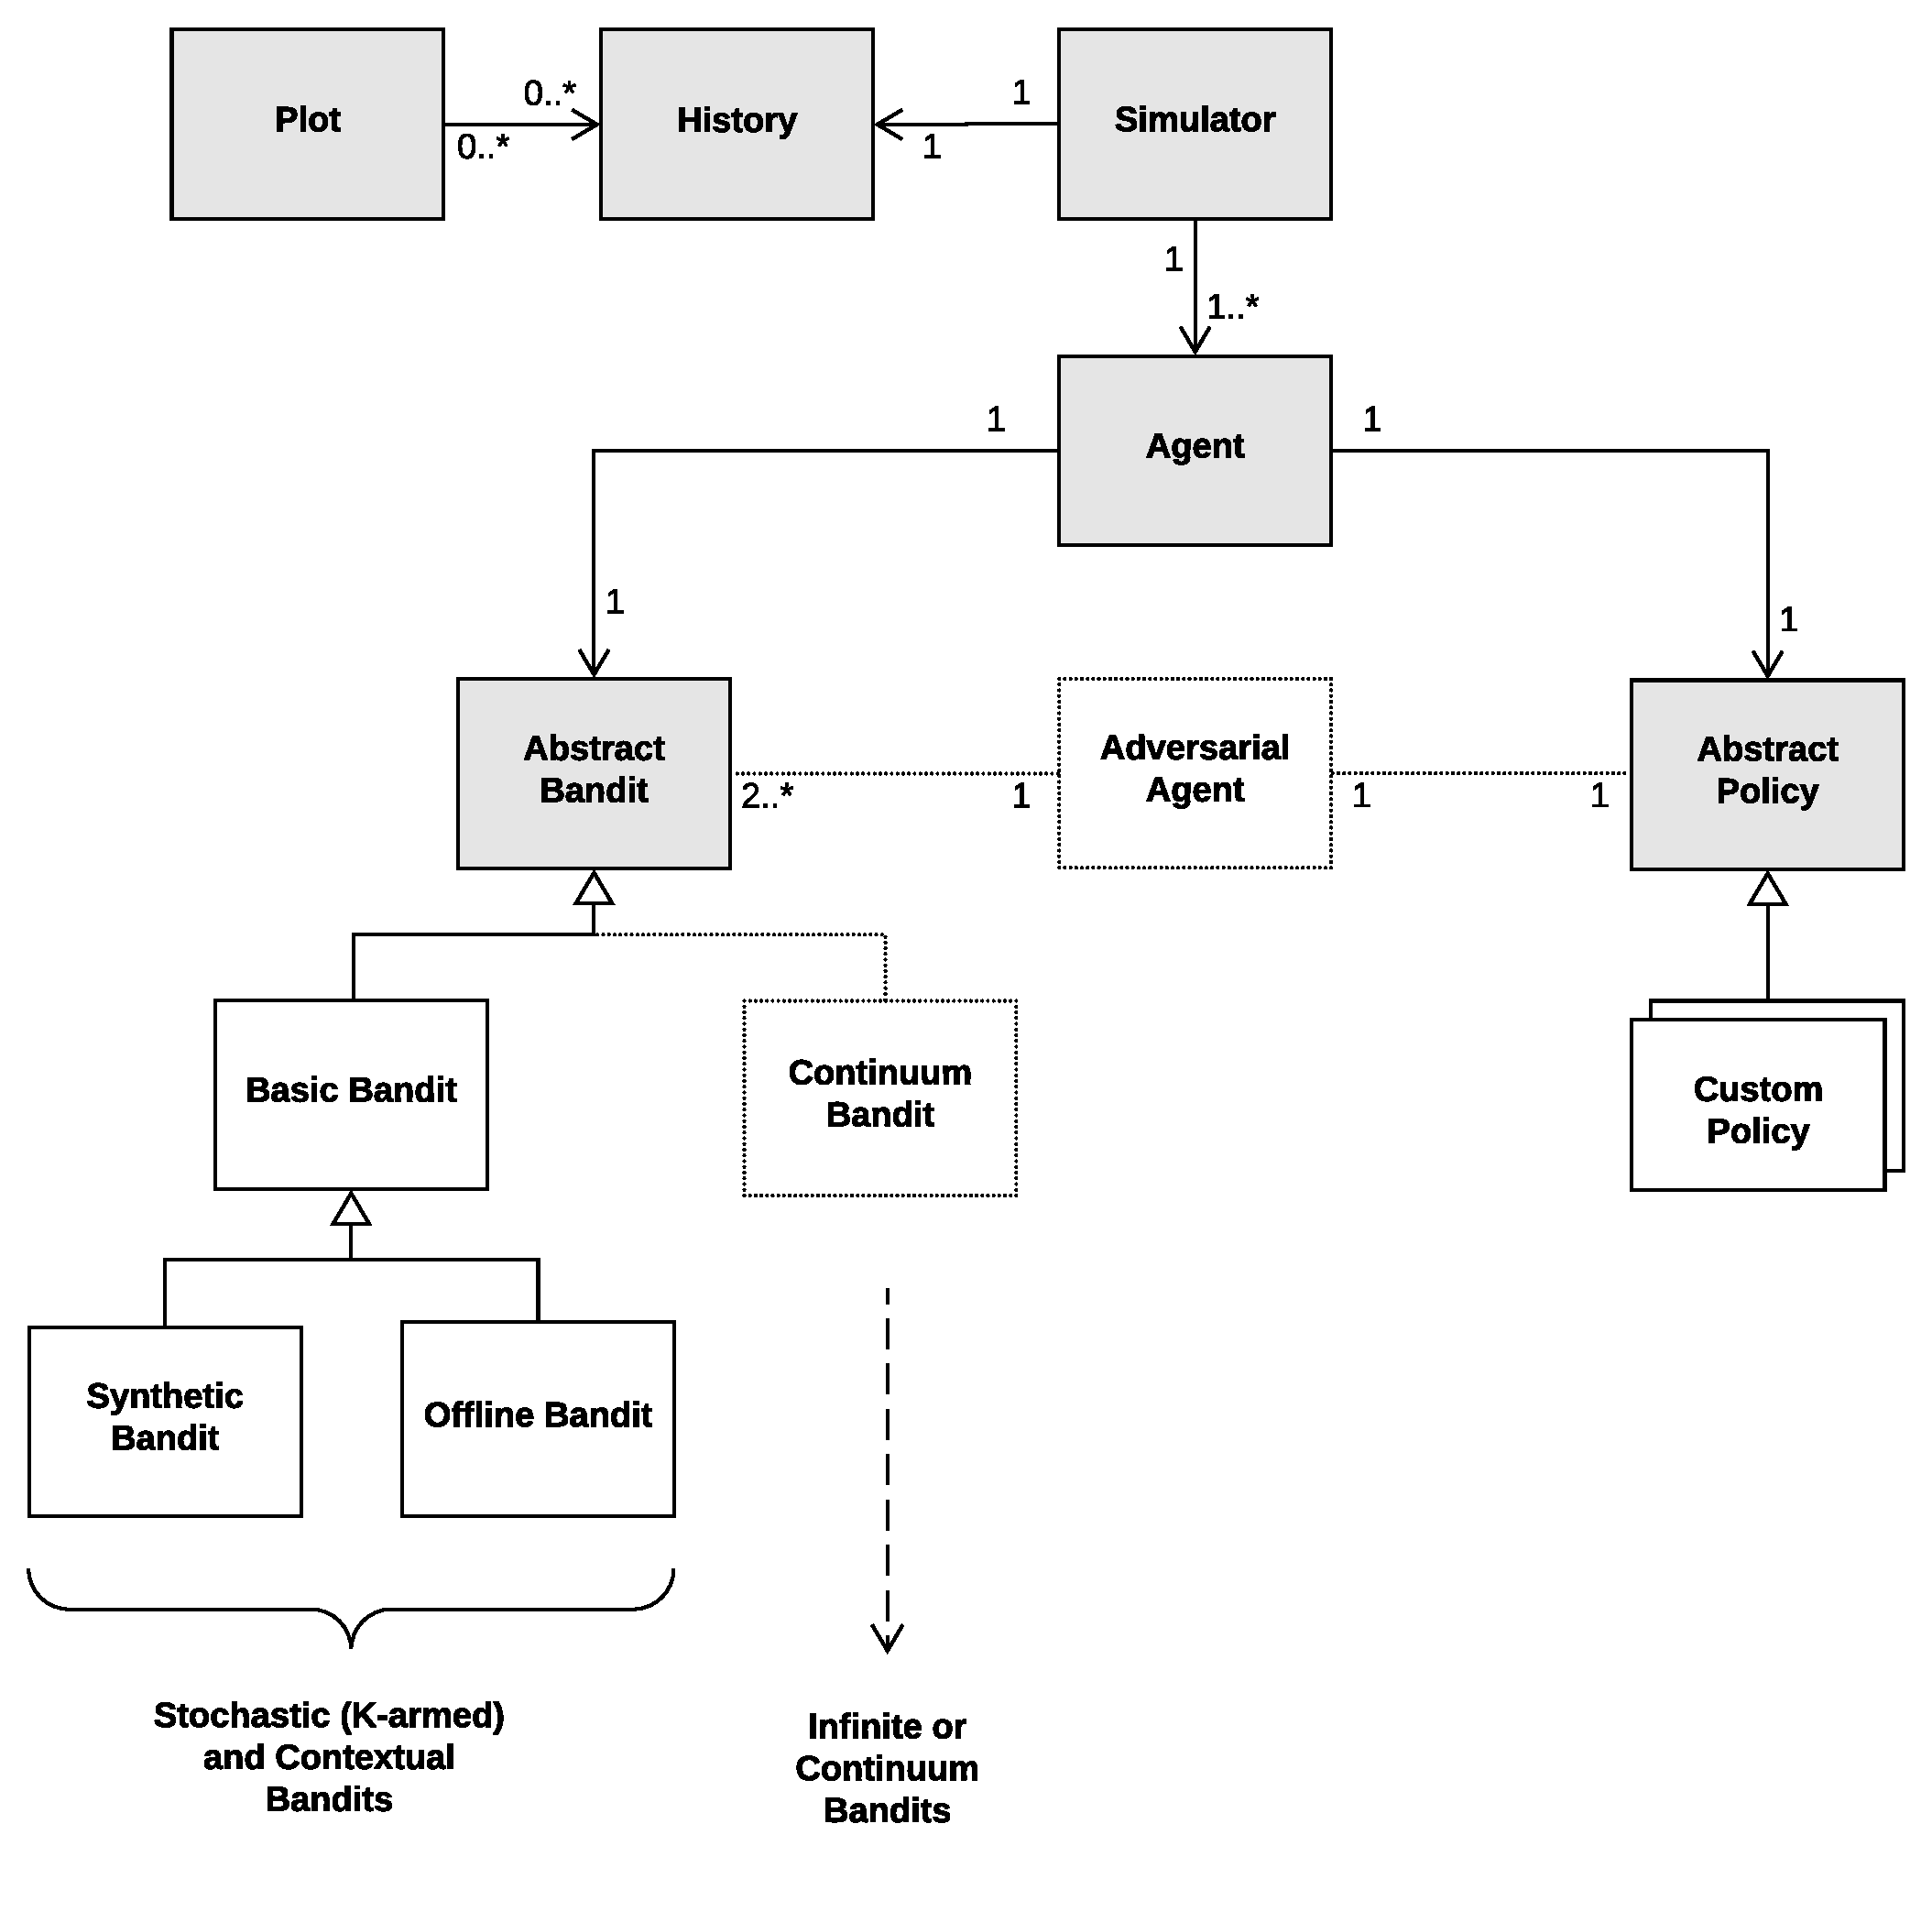
\includegraphics[width=.99\textwidth]{fig/contextual_class}
    \label{fig:contextual_class}
      \caption{\pkg{contextual} UML Class Diagram}
\end{figure}

\begin{figure}[H]
  \centering
    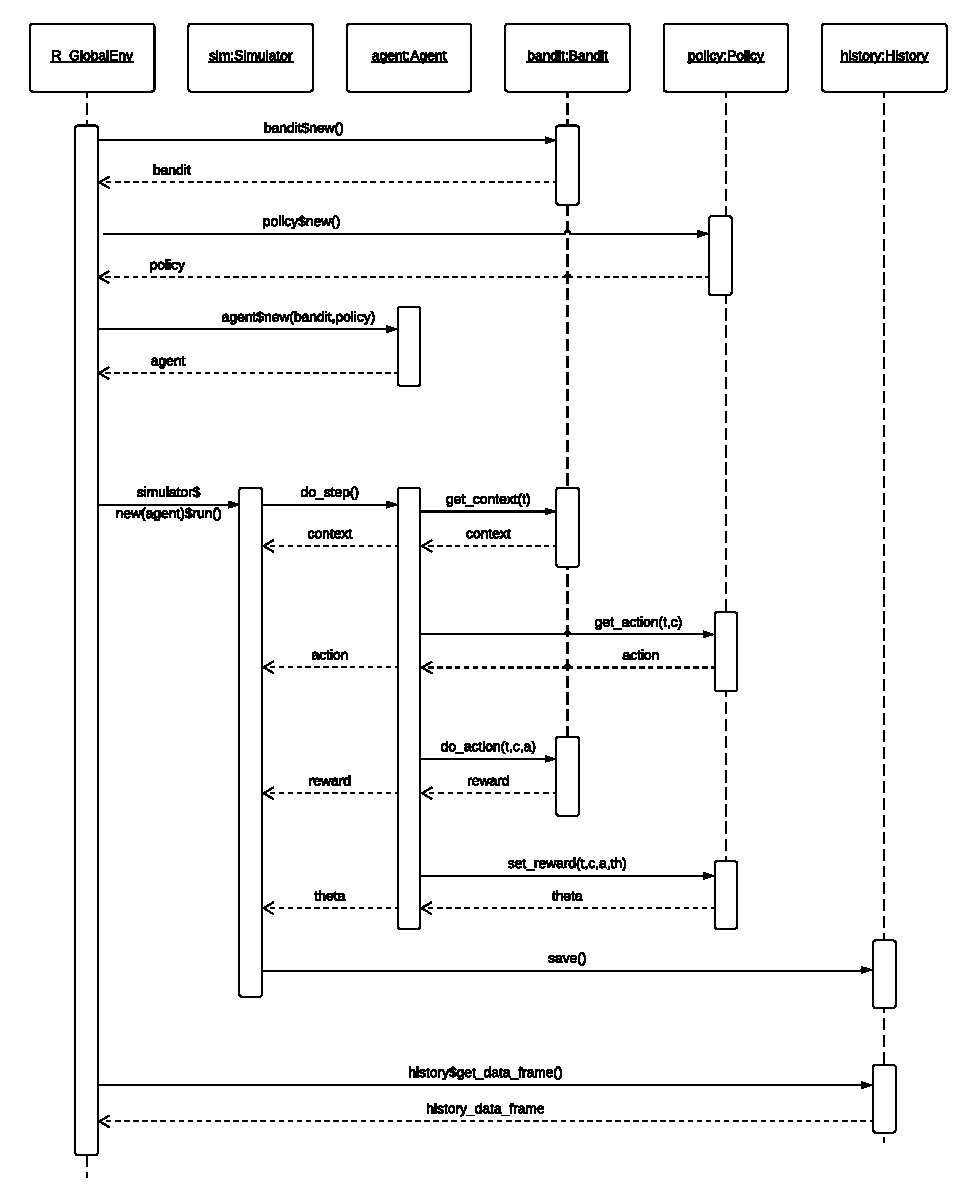
\includegraphics[width=.99\textwidth]{fig/contextual_sequence}
    \label{fig:contextual_sequence}
      \caption{\pkg{contextual} UML Sequence Diagram}
\end{figure}

\section{Acknowledgments}

Thanks go to my colleagues at the Jheronimus Academy of Data Science and Tilburg University!

%\bibliographystyle{apacite}
\bibliography{jss}

\end{document}
